\documentclass[twoside]{article}
\usepackage[utf8]{inputenc}
\usepackage[ngerman]{babel}
\usepackage{libertine}
\usepackage[a4paper]{geometry}
\usepackage{pdfpages}
\usepackage{parskip}
\usepackage{amsmath, amsthm, amssymb, commath, mathtools}
\usepackage{cancel}
\usepackage{physics}
\usepackage{nicefrac}
\usepackage{booktabs}
\usepackage{tabularx}
\usepackage{tabu}
\usepackage{enumitem}
\usepackage{graphicx}
\graphicspath{{./plots/}{./images/}}
\usepackage{wrapfig}
\usepackage{caption}
\usepackage{float}
\usepackage{minted}
\usepackage{appendix}
\usepackage{icomma}
\usepackage{multirow}
\usepackage{multicol}
\usepackage{footmisc}
\usepackage[separate-uncertainty=true]{siunitx}
\sisetup{locale = DE}
\usepackage{xcolor}

\usepackage{csquotes}
\MakeOuterQuote{"}
\renewcommand{\ttdefault}{cmtt}

\usepackage{hyperref}
\usepackage{bookmark}
% https://tex.stackexchange.com/a/33701
\makeatletter
    \newcommand{\nonum}[0]{%
        \let\@oldseccntformat\@seccntformat %
        \renewcommand\@seccntformat[1]{}%
        }
    \newcommand{\resnum}[0]{\let\@seccntformat\@oldseccntformat}
\makeatother

\usepackage{chngcntr}
\counterwithin{figure}{section}

\newcommand{\versuch}[0]{MZI}
\newcommand{\versuchLang}[0]{Mach-Zender-Interferometer}

\hypersetup{
	pdftitle={P3A -- \versuch{} Auswertung},
	pdfauthor={Yudong Sun},
	bookmarksnumbered=true,
	bookmarksopen=true,
	bookmarksopenlevel=2,
	pdfstartview=Fit,
	pdfpagemode=UseOutlines,
	colorlinks=true,
	linkcolor=black,
	filecolor=magenta,      
	urlcolor=blue
}
\urlstyle{same}

\title{\versuch{} -- \versuchLang \\ Auswertung}
\author{Yudong Sun\\Gruppe I4}

\usepackage{fancyhdr}
\pagestyle{fancy}
\fancyhf{}
\fancyhead[RO]{Yudong Sun}
\fancyhead[LO]{Auswertung -- \versuch}
\fancyhead[LE]{Yudong Sun}
\fancyhead[RE]{Auswertung -- \versuch}
\cfoot{\thepage}

% Custom Defs
\newcommand*{\ra}[1]{\renewcommand{\arraystretch}{#1}}
\newcommand*{\maxi}[1]{\text{max}\left(#1\right)}
\newcommand*{\mini}[1]{\text{min}\left(#1\right)}
\newcommand*{\todo}[1]{\textcolor{red}{TODO: #1}}
\newcommand*{\iu}[1]{\textit{\underline{#1}}}
\newcommand*{\gnuplot}[0]{\texttt{gnuplot}}
\newcommand*{\captionbr}[0]{\\\rule{\textwidth}{0pt}\\\vspace{-\baselineskip}}
\newcommand*{\sigfig}[1]{\hspace{0.5cm}\text{(#1 sig. Zif.)}}
\newcommand*{\pbrace}[1]{\left(#1\right)}
\newcommand*{\sbrace}[1]{\left[#1\right]}
\newcommand*{\bDelta}[1]{\pbrace{\Delta #1}}
\newcommand*{\overbar}[1]{\overline{\raisebox{0pt}[1.2\height]{$#1$}}} % https://tex.stackexchange.com/a/87615

% \addto\captionsngerman{
%     \let\oldfigname\figurename
%     \renewcommand{\figurename}{[\oldfigname}
%     \let\oldthefig\thefigure
%     \renewcommand{\thefigure}{\oldthefig]}
% } % https://tex.stackexchange.com/a/17490
% https://tex.stackexchange.com/a/101624 new line in caption

% Gaußsche Fehler Erzeuger
\makeatletter
    \newcommand{\gausserror}[2]{% \gausserror{G}{faktoren}
        \sqrt{%
            \@tempswafalse
            \@for\factor:=#2
            \do{
                \if@tempswa+%
                \else%
                    \@tempswatrue%
                \fi%
                \left(\pdv{#1}{\factor}\Delta\factor\right)^2%
            }%
        }
    }
\makeatother
% https://tex.stackexchange.com/a/59912
% https://riptutorial.com/latex/example/28657/loops---repeating-things

% Add quad
\makeatletter
    \newcommand{\addquad}[1]{% \gausserror{G}{faktoren}
        \sqrt{%
            \@tempswafalse
            \@for\factor:=#1
            \do{
                \if@tempswa+%
                \else%
                    \@tempswatrue%
                \fi%
                \left(\Delta\factor\right)^2%
            }%
        }
    }
\makeatother

% rej quad
\makeatletter
    \newcommand{\relquad}[1]{% \gausserror{G}{faktoren}
        \sqrt{%
            \@tempswafalse
            \@for\factor:=#1
            \do{
                \if@tempswa+%
                \else%
                    \@tempswatrue%
                \fi%
                \left(\frac{\Delta\factor}{\factor}\right)^2%
            }%
        }
    }
\makeatother

% / Custom Defs

\begin{document}

\maketitle

% Einstellungen
\nonum
\numberwithin{equation}{section}
% / Einstellungen

\section{Teilversuch 1: Aufbau des Foldscopes}
	\begin{tabularx}{\textwidth}{l p{1mm} X}
		\toprule
		\tou{Versuchsziel} && Aufbau des Foldscopes \\
		\tou{Messmethode} && Augenmaß \\
		\bottomrule
	\end{tabularx}
	\subsection{Linsengleichung für eine biconvexe Linse}
		Für eine Linse mit brechenden Kugelflächen gilt die allgemeine Linsenschleiferformel \citep{kling_96_nodate}:
		\begin{equation}
			\frac{1}{f} = \left(\frac{n_L}{n_M} - 1\right)\left(\frac{1}{R_1} - \frac{1}{R_2} + \frac{\left(\frac{n_L}{n_M} - 1\right)d}{\frac{n_L}{n_M}R_1R_2}\right)
		\end{equation}
		mit \hspace{1cm}
		\begin{tabular}{ll}
			$f$   & Effektive Brennweite der Linse vom Zentrum \\
			$n_L$ & Brechungsindex vom der Linse \\
			$n_M$ & Brechungsindex von das umgebende Medium \\
			$R_1$ & Krümmungsradius der Eintrittsfläche (mit Vorzeichen) \\
			$R_2$ & Krümmungsradius der Austrittsfläche (mit Vorzeichen) \\
			$d$   & Dicke der Linse
		\end{tabular}

		Für eine biconvexe Linse ist $R_1 > 0$ und $R_2 < 0$. Da wir die Linse nur im Luft verwenden, ist $n_M \approx 1$, wie wir im Versuch MZI bestätigt haben. Schreibe $\frac{n_L}{n_M}$ als $n$, dann erhalten wir:
		\begin{equation}
			\frac{1}{f} = \left(n - 1\right)\left(\frac{1}{R_1} - \frac{1}{R_2} + \frac{\left(n - 1\right)d}{nR_1R_2}\right)
		\end{equation}
		Wir verwenden in diesem Versuch eine Kugellinse, somit ist $\abs{R_1} = \abs{R_2} = R$ und $d = 2R$. Somit ergibt sich:
		\begin{align}
			\frac{1}{f} 
			&= \left(n - 1\right)\left(\frac{1}{R} + \frac{1}{R} - \frac{\left(n - 1\right)(2R)}{nR^2}\right) \notag \\ 
			&= \left(n - 1\right)\left(\frac{2}{R} - \frac{\left(2n - 2\right)R}{nR^2}\right) \notag \\
			&= \left(n - 1\right)\left(\frac{\cancel{2n} - \left(\cancel{2n} - 2\right)\cancel{R}}{nR\cancel{^2}}\right) \notag \\
			&= \frac{2(n-1)}{nR}
		\end{align}
		Daraus ergibt sich die effektive Brennweite:
		\begin{align}
			f = \frac{nR}{2(n-1)} = \frac{nD}{4(n-1)} \label{eqn:focallength}
		\end{align}
		wobei $D$ der Durchmesser ist. 

		Es gilt außerdem unter der paraxiellen Näherung die Gleichung:
		\begin{align}
			\frac{1}{f} = \frac{1}{g} + \frac{1}{b}
		\end{align}
		mit \hspace{1cm}
		\begin{tabular}{ll}
			$f$   & Effektive Brennweite der Linse vom Zentrum \\
			$g$   & Gegenstandsweite \\
			$b$   & Bildweite
		\end{tabular}

	\subsection{Fotoprotokoll des Aufbaus}
		Anhand der beiliegenden Anleitung (Siehe Anhang \ref{appdx:anleitung}) wurde das Foldscope aufgebaut. Die hier dokumentierte Schritten entsprechen die Schritten in der Anleitung.
		\vfill
		\begin{center}
			\begin{tabular}{*{3}{l}}
				% \toprule
				\multicolumn{1}{l|}{Schritt 1} & Schritt 2 & $\rightarrow$\\
				\midrule
				\multicolumn{1}{l|}{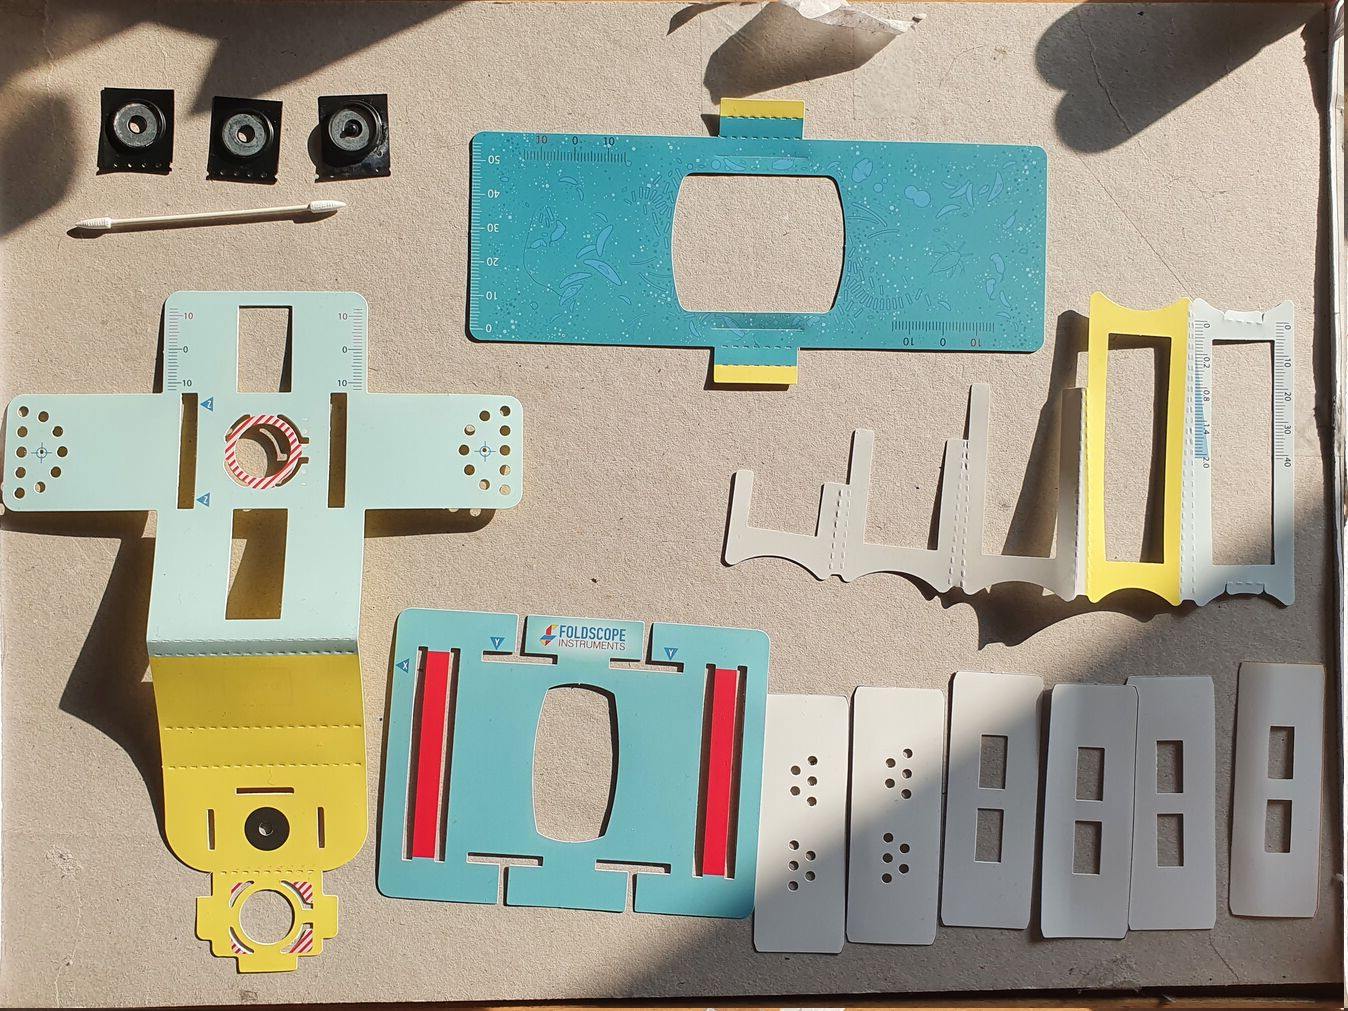
\includegraphics[width=0.3\textwidth]{images/aufbau/1_1.jpg}} & 
				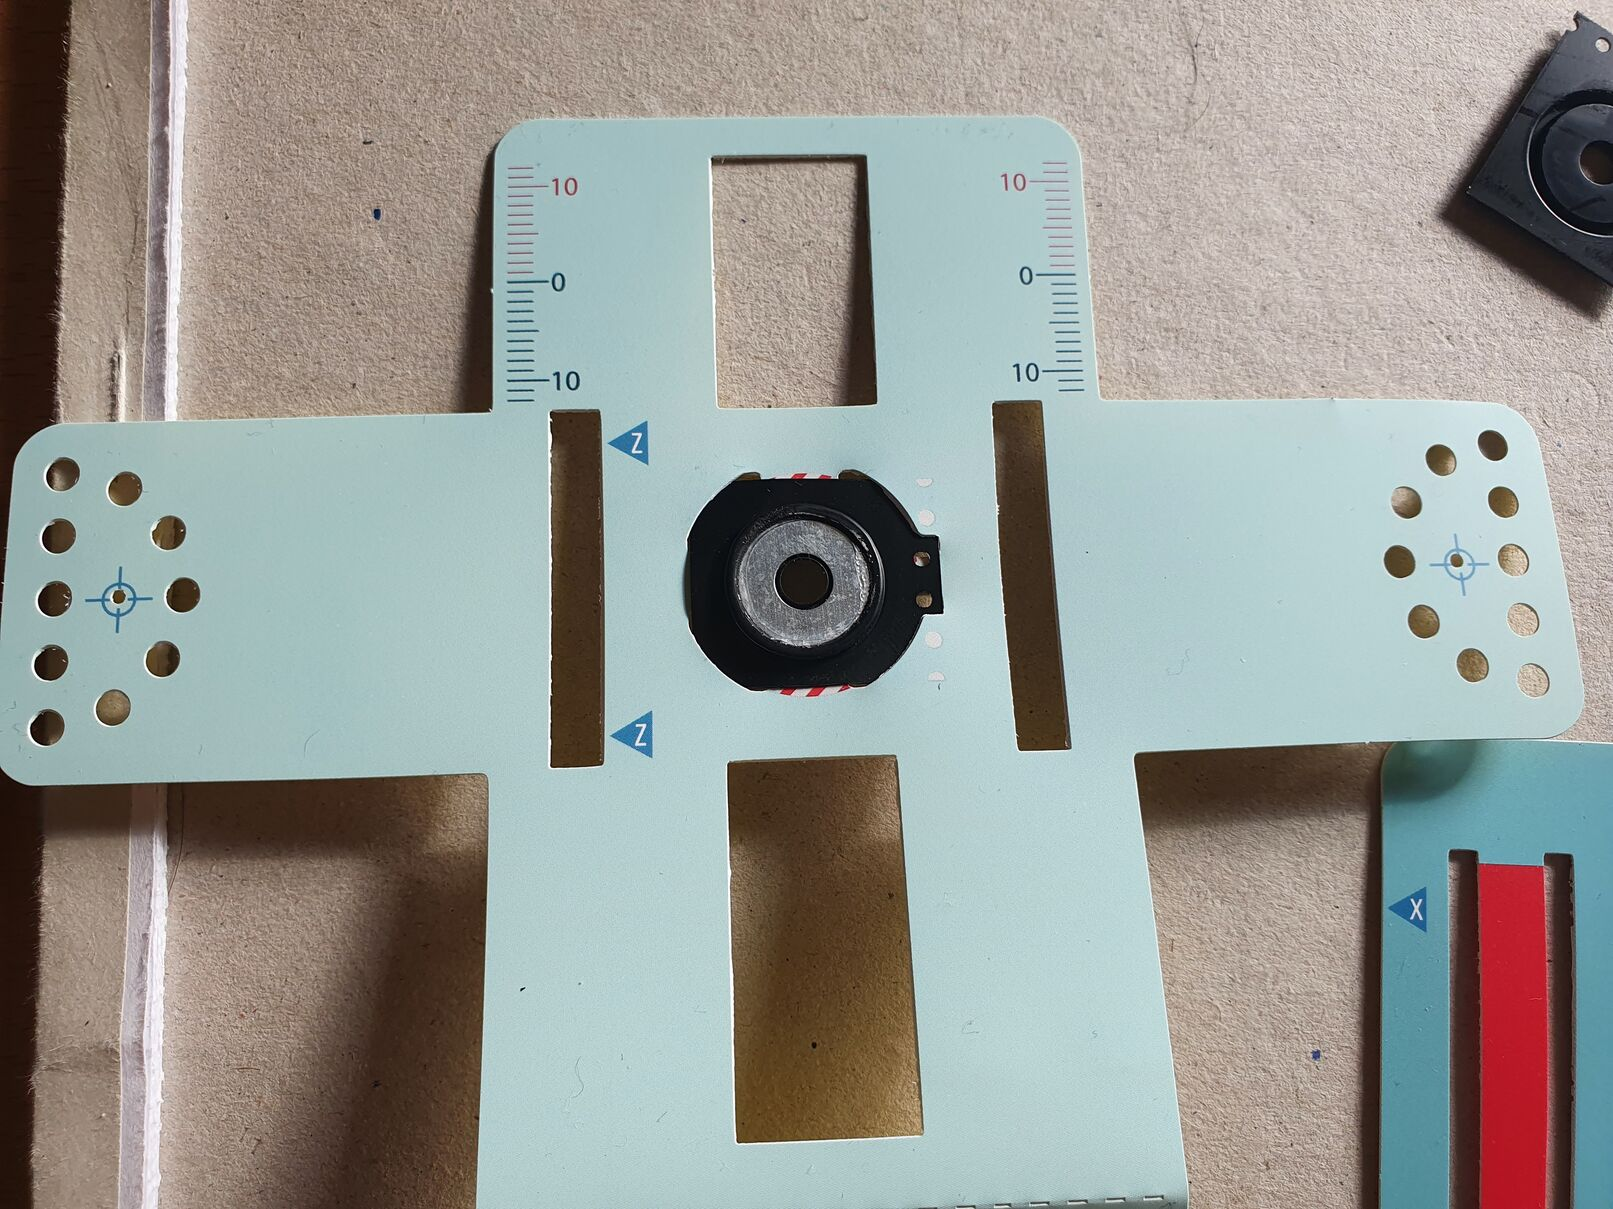
\includegraphics[width=0.3\textwidth]{images/aufbau/2_1.jpg} & 
				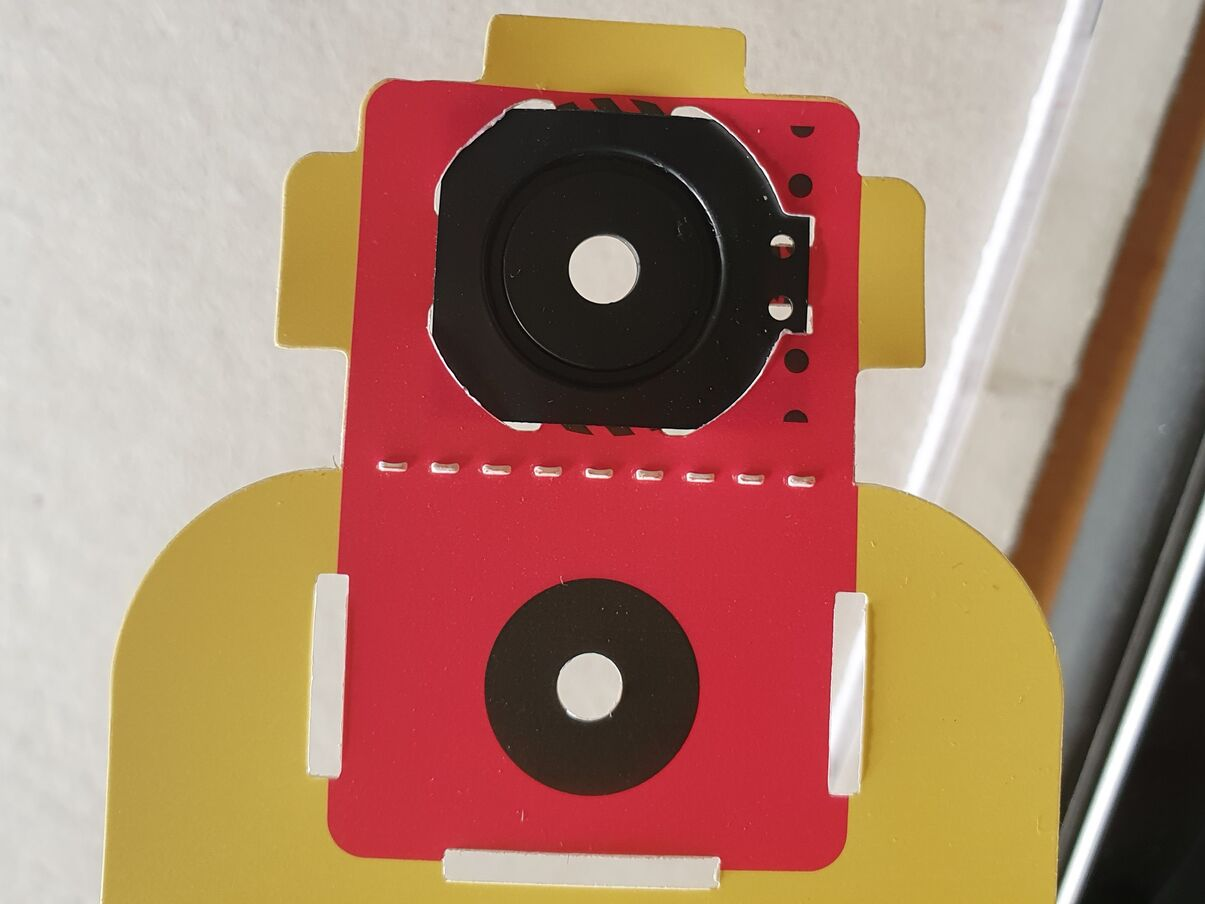
\includegraphics[width=0.3\textwidth]{images/aufbau/2_2.jpg} \\
				% \bottomrule 
				\\[-0.5em]
				% \toprule
				$\rightarrow$ & \multicolumn{1}{l|}{$\rightarrow$} & Schritt 3 \\
				\midrule
				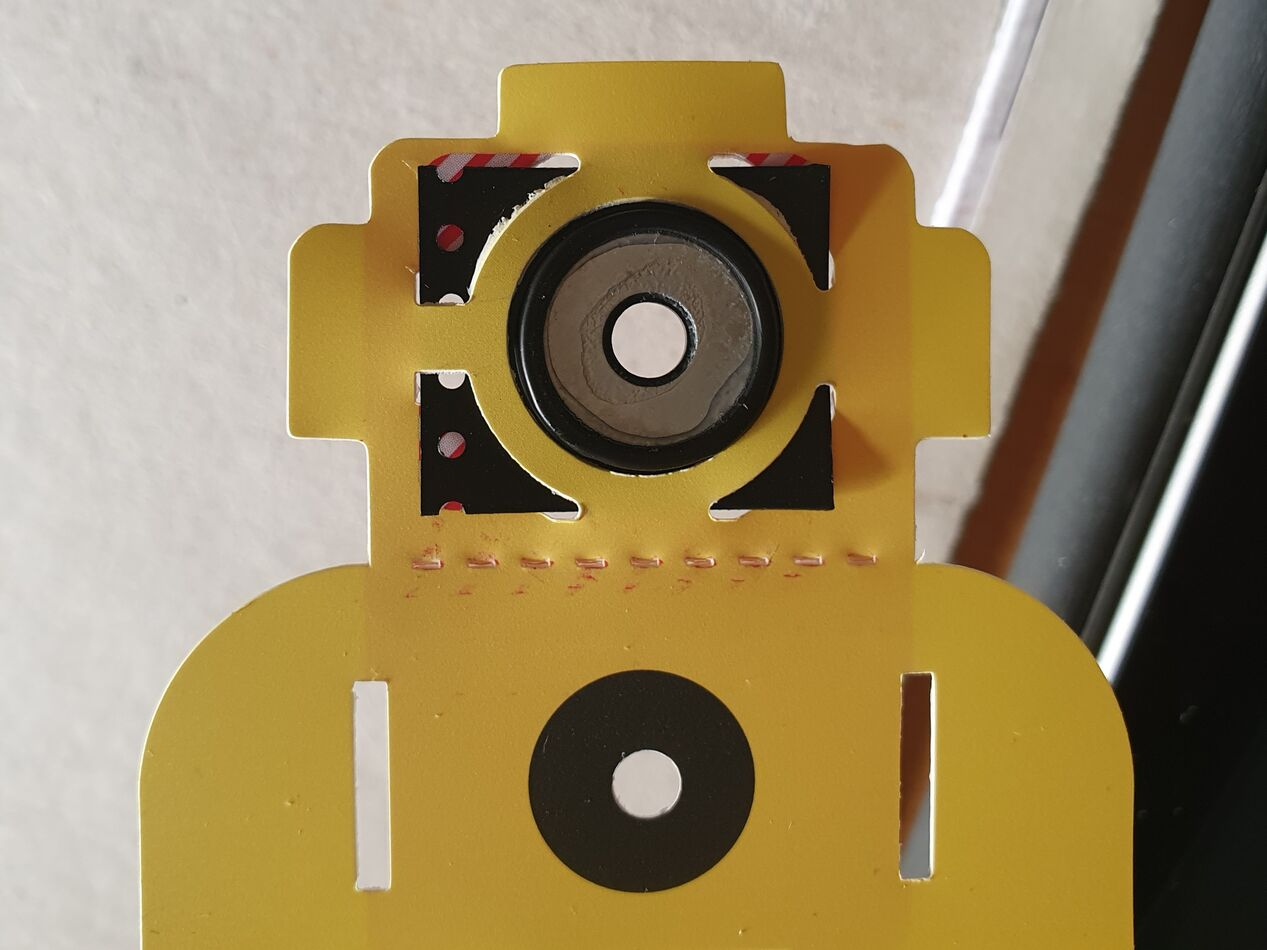
\includegraphics[width=0.3\textwidth]{images/aufbau/2_3.jpg} &
				\multicolumn{1}{l|}{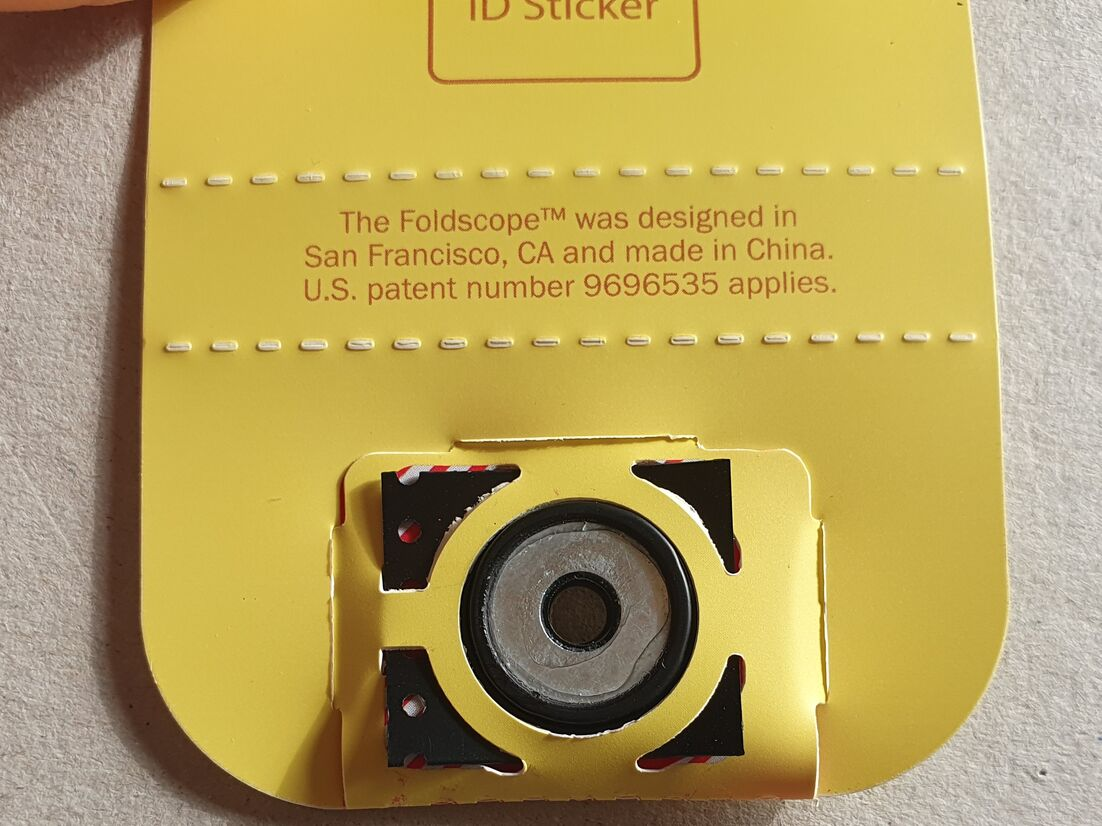
\includegraphics[width=0.3\textwidth]{images/aufbau/2_4.jpg}} &
				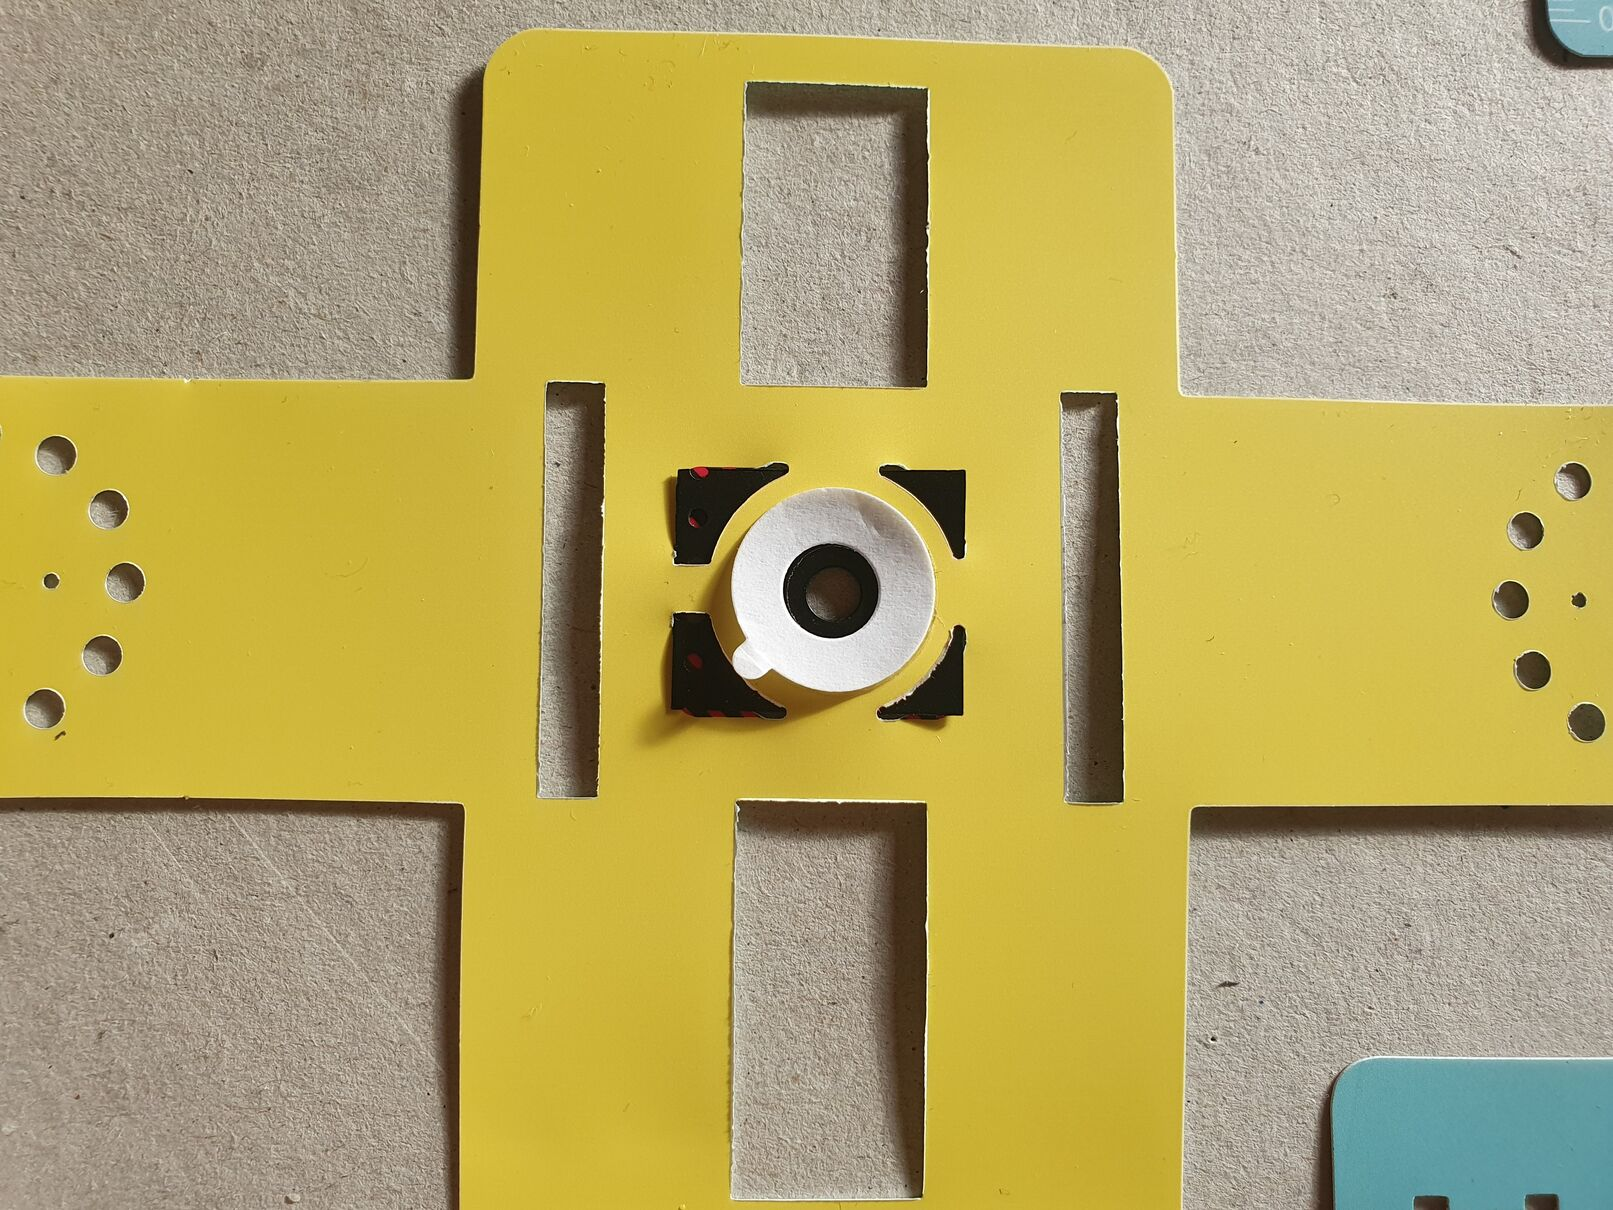
\includegraphics[width=0.3\textwidth]{images/aufbau/3_1.jpg} 
				\\
				% \bottomrule
				\\[-0.5em]
				% \toprule
				$\rightarrow$ & \multicolumn{1}{l|}{$\rightarrow$} & Schritt 4 \\
				\midrule
				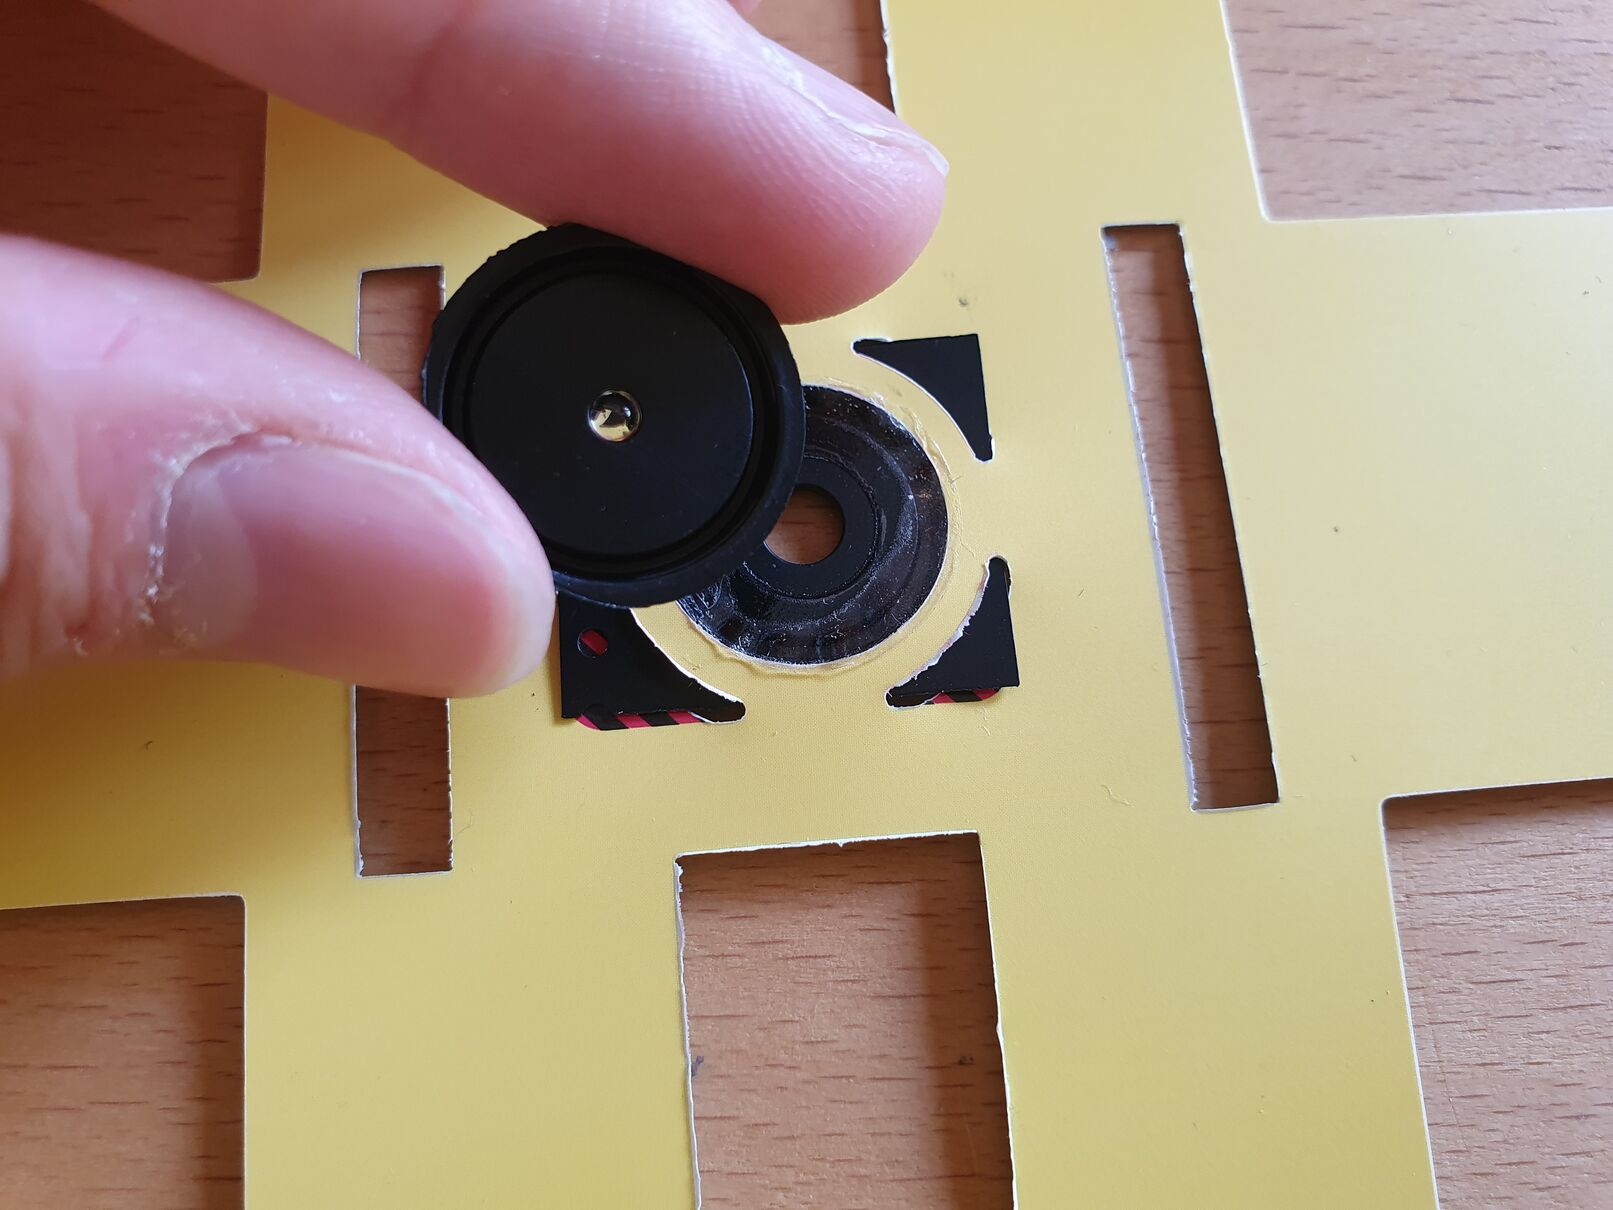
\includegraphics[width=0.3\textwidth]{images/aufbau/3_2.jpg} &
				\multicolumn{1}{l|}{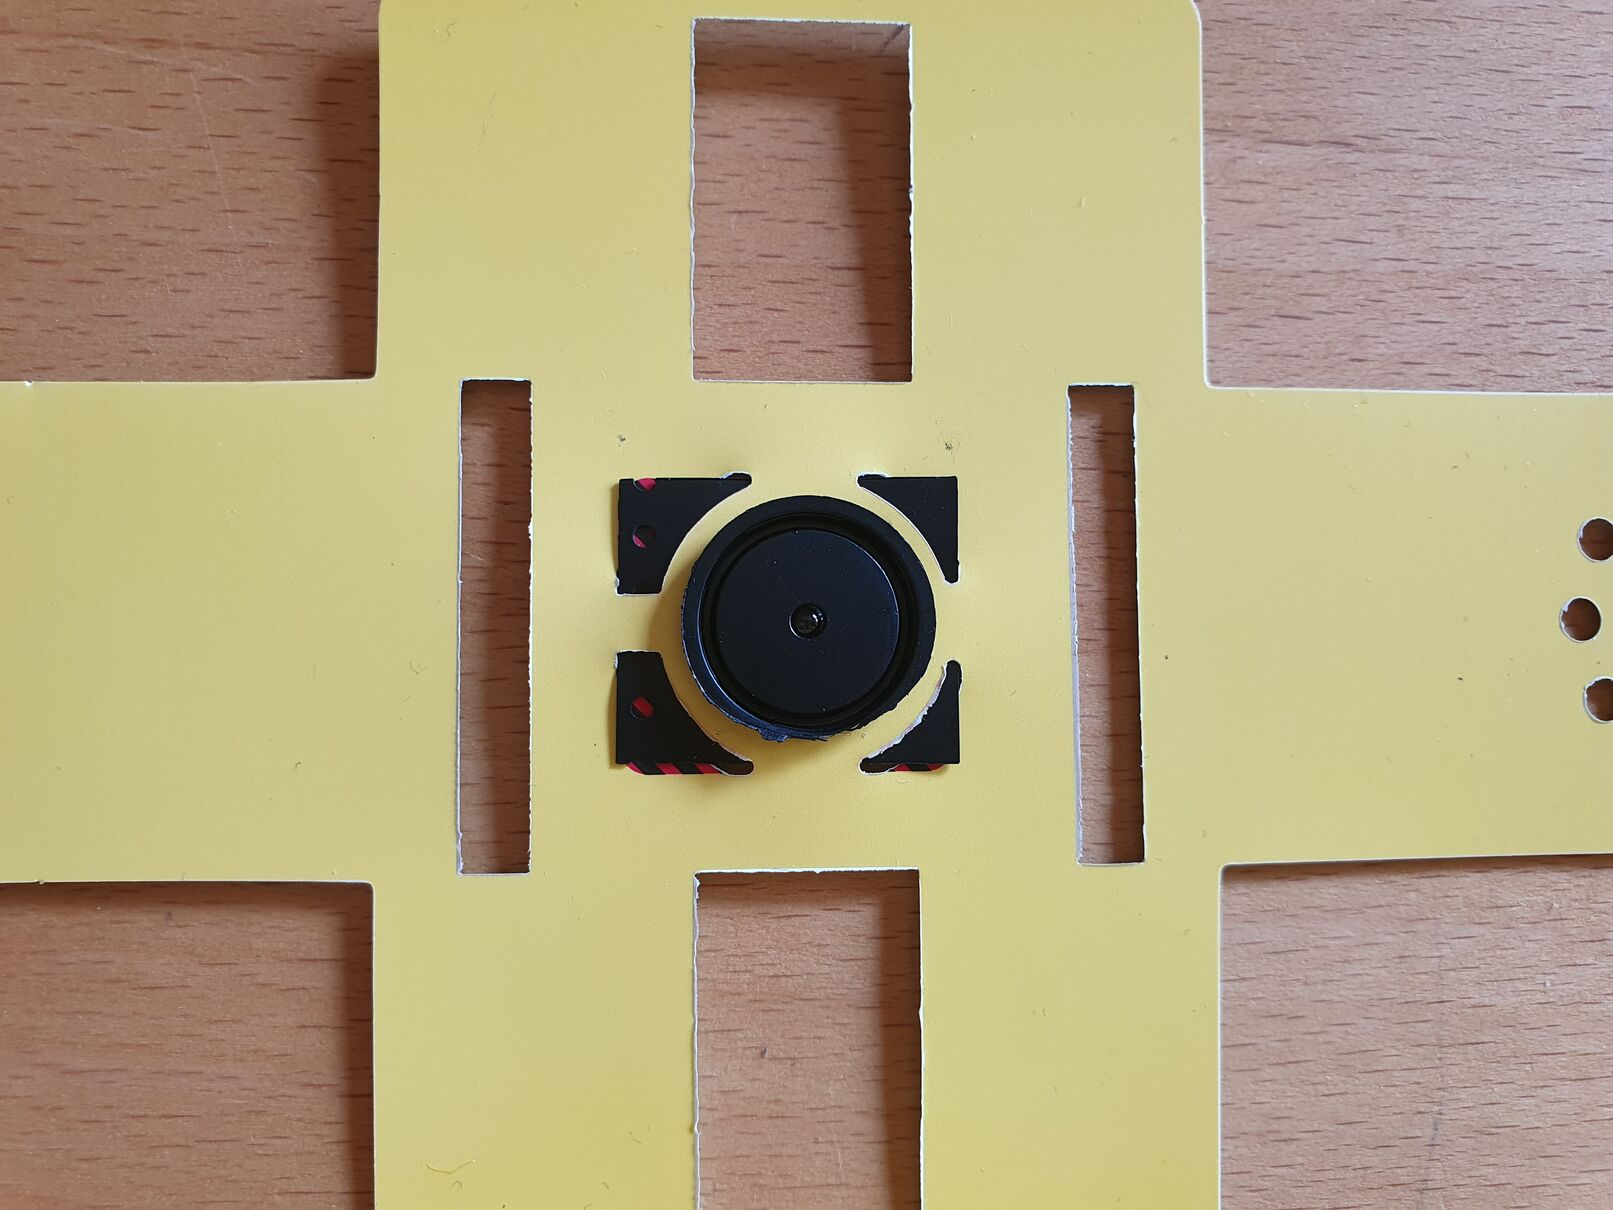
\includegraphics[width=0.3\textwidth]{images/aufbau/3_3.jpg}} &
				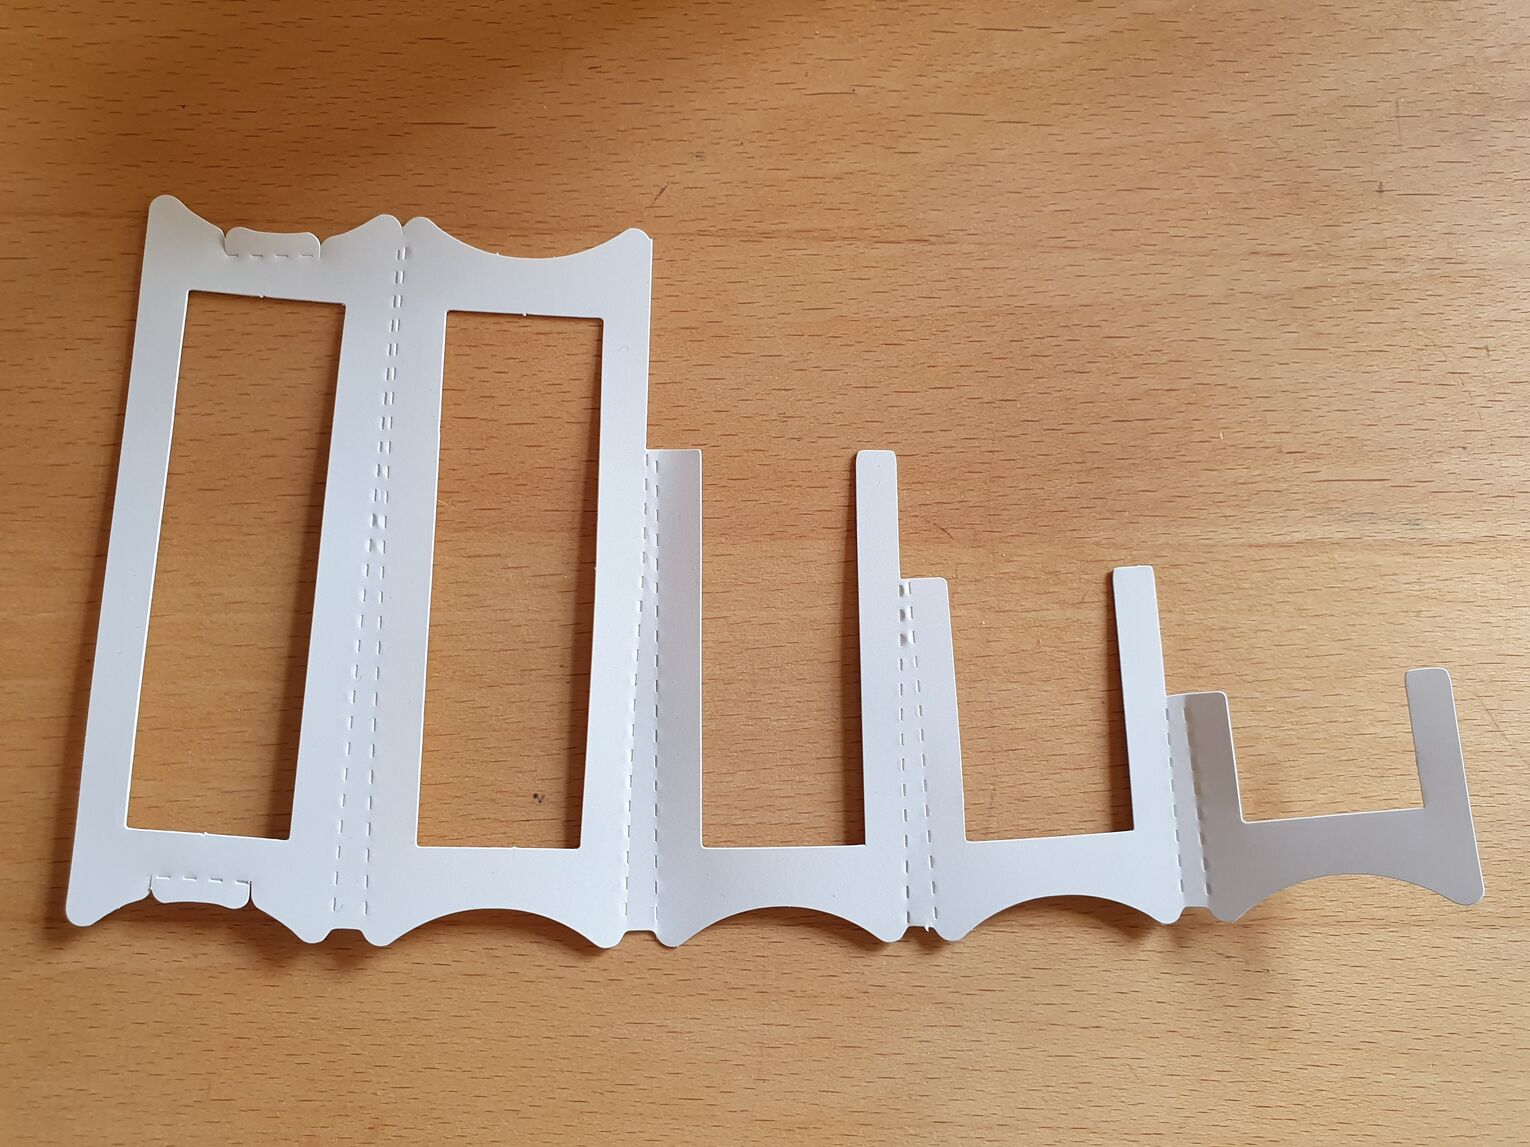
\includegraphics[width=0.3\textwidth]{images/aufbau/4_1.jpg} 
				\\
				% \bottomrule
			\end{tabular}
		\end{center}
		\vfill
		\newpage
		\begin{center}
			\begin{tabular}{l|l|l}
				% \toprule
				\multicolumn{1}{l}{$\rightarrow$} & $\rightarrow$ & Schritt 5 \\
				\midrule
				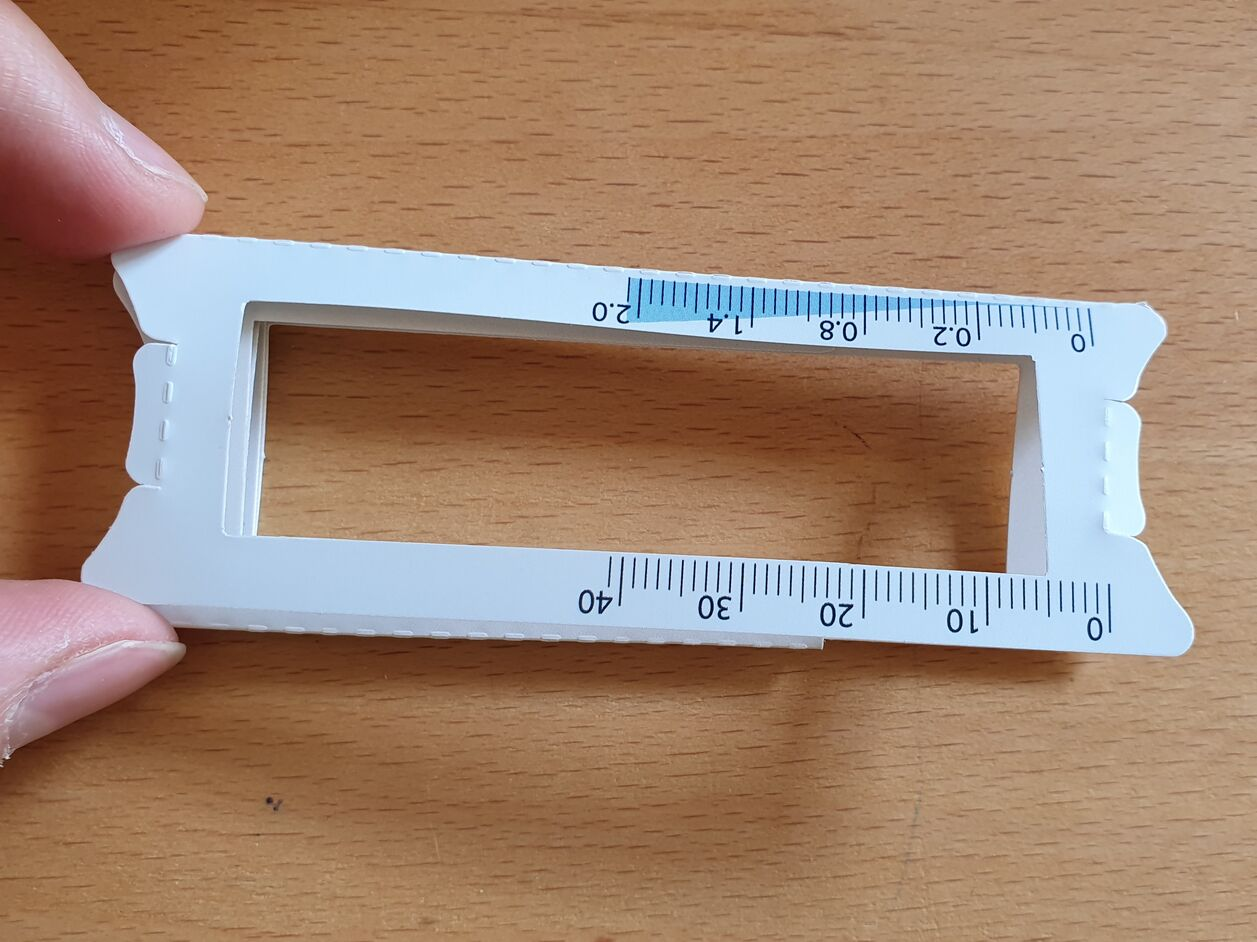
\includegraphics[width=0.3\textwidth]{images/aufbau/4_2.jpg} &
				
\includegraphics[width=0.3\textwidth]{images/aufbau/4_3.jpg} &
				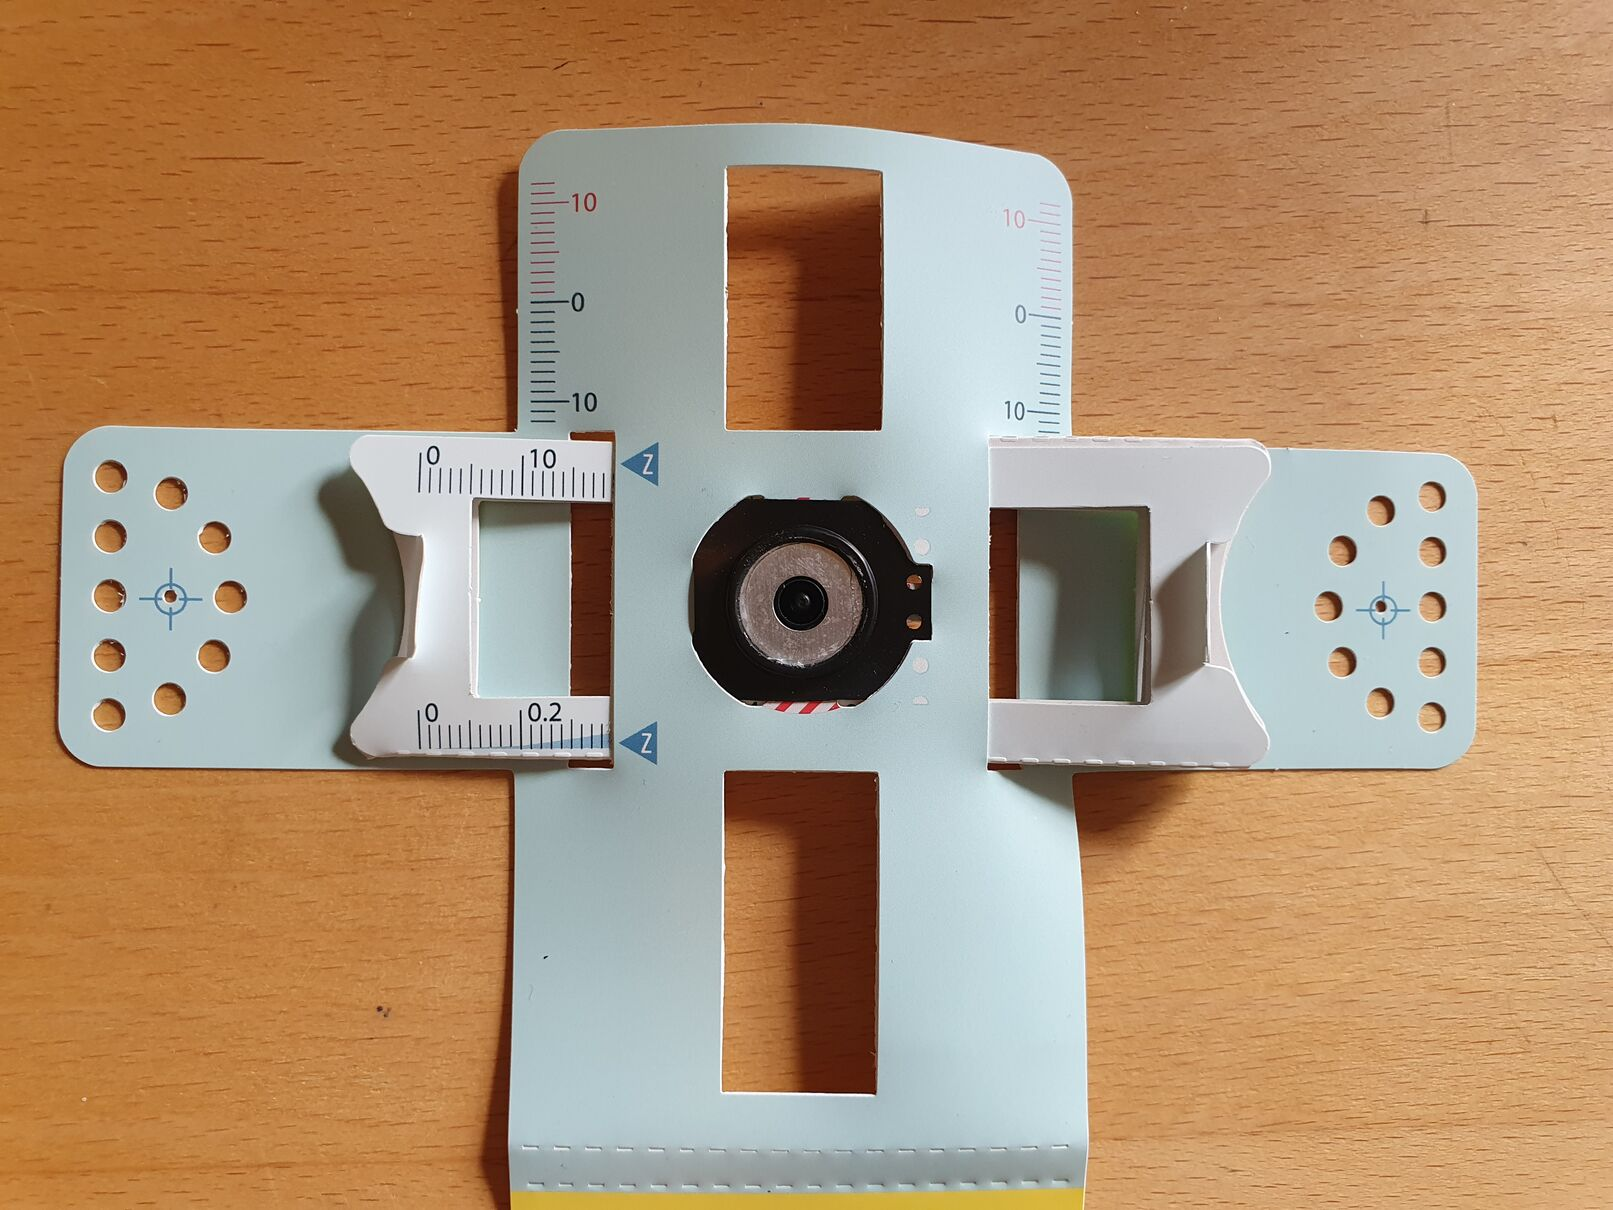
\includegraphics[width=0.3\textwidth]{images/aufbau/5.jpg} \\
				% \bottomrule
				\multicolumn{3}{l}{} \\[-0.5em]
				% \toprule
				Schritt 6 & Schritt 7 & Schritt 8  \\
				\midrule
				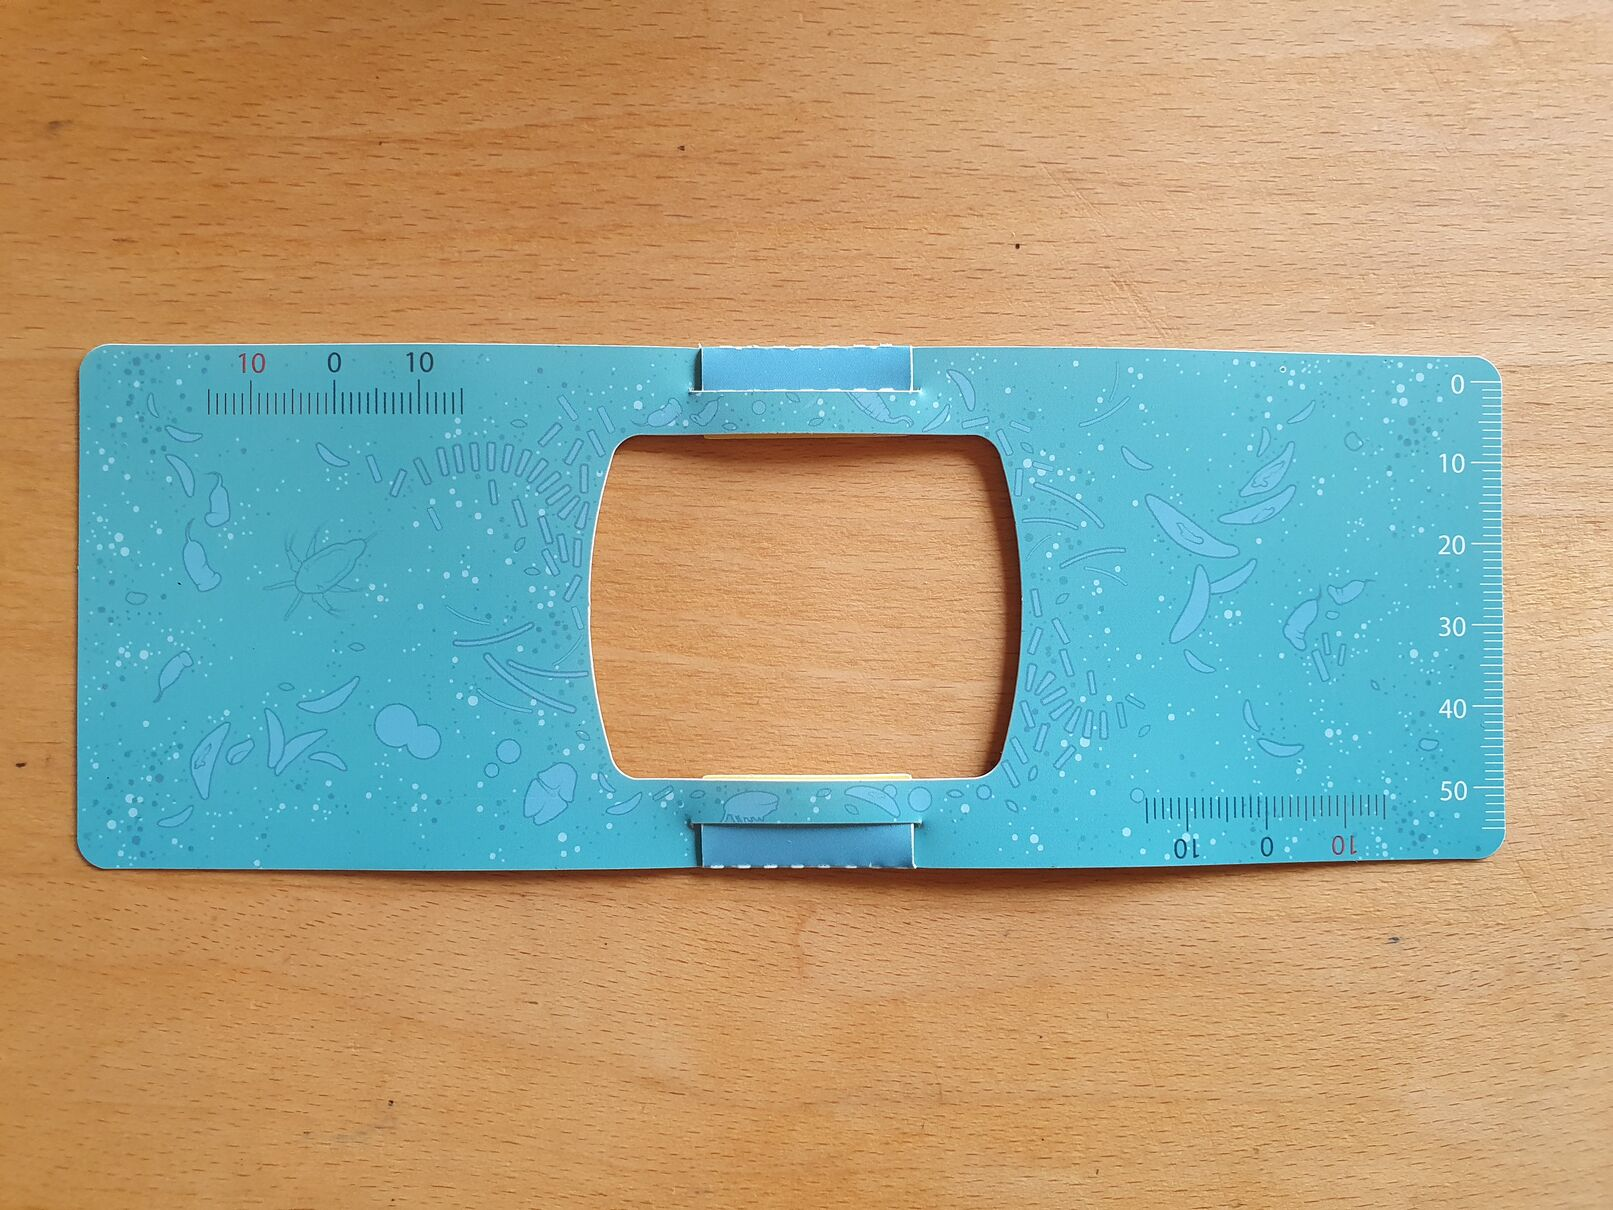
\includegraphics[width=0.3\textwidth]{images/aufbau/6.jpg} &
				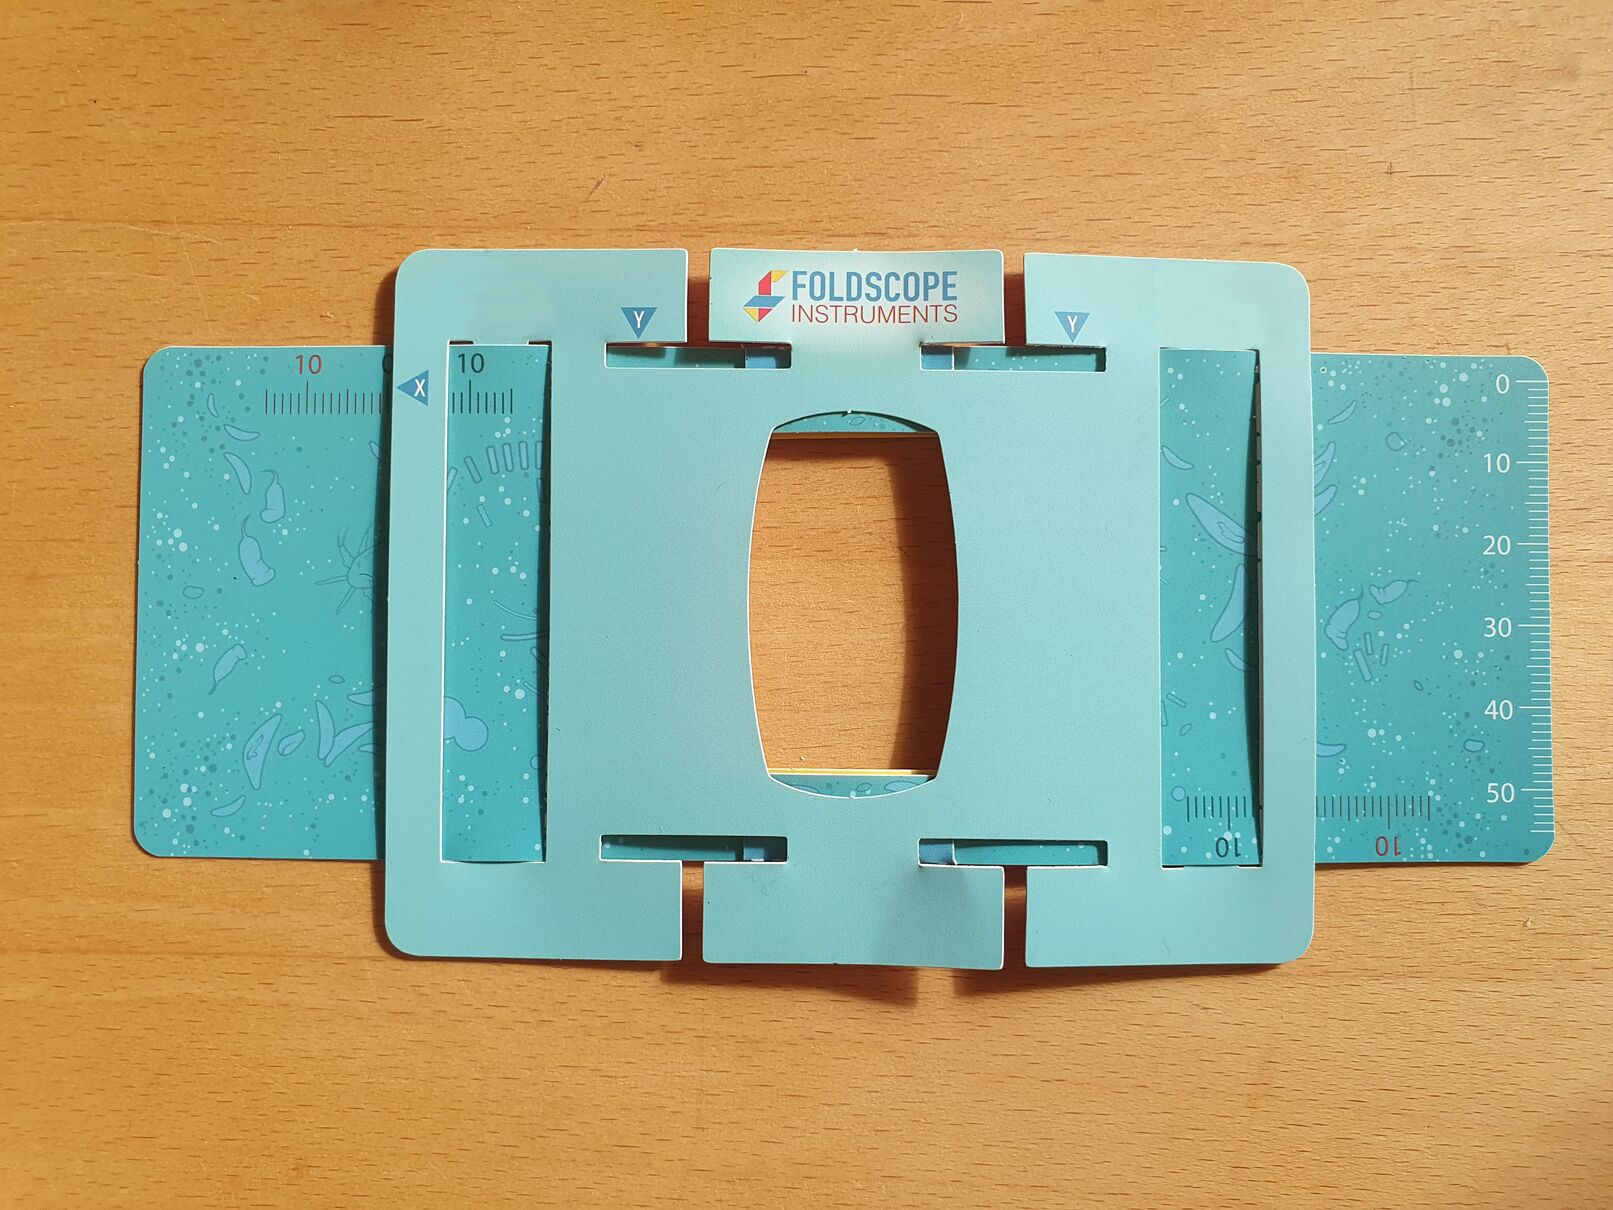
\includegraphics[width=0.3\textwidth]{images/aufbau/7.jpg} &
				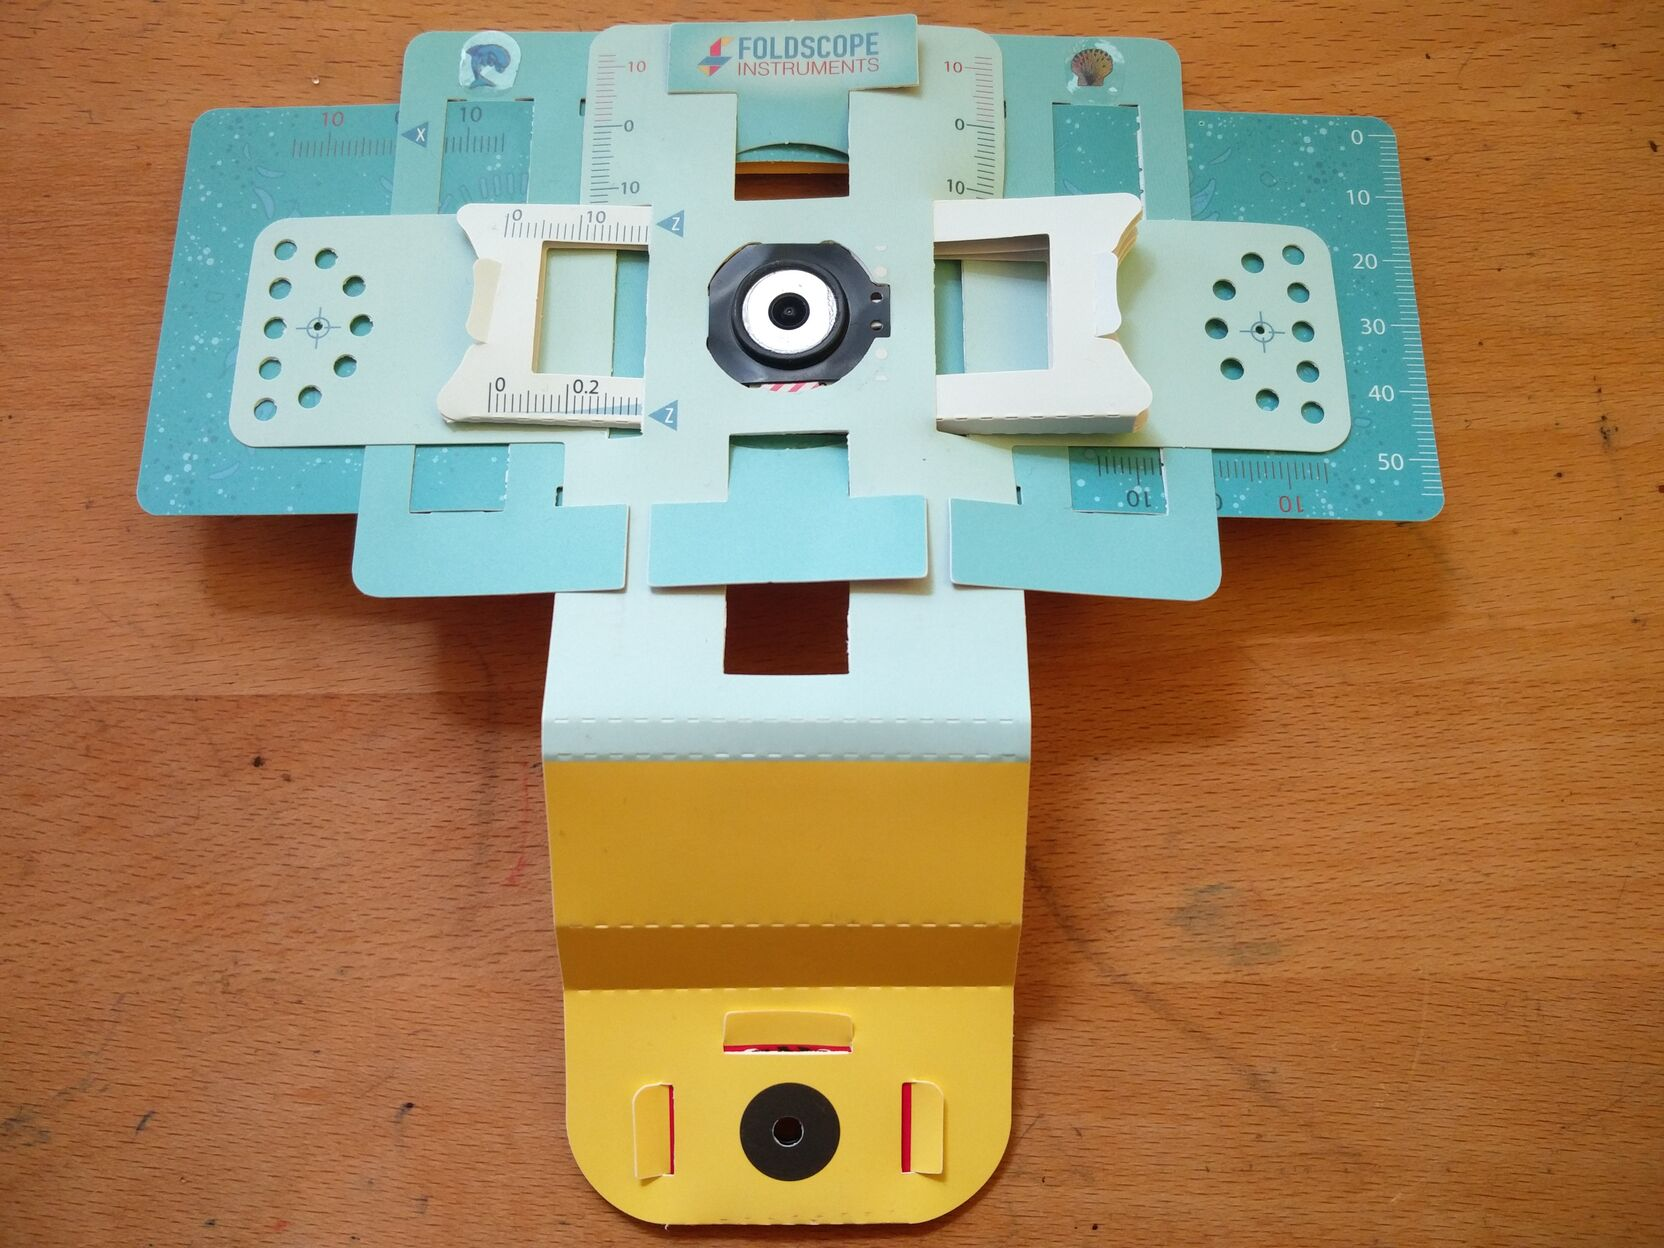
\includegraphics[width=0.3\textwidth]{images/aufbau/8.jpg} \\
				% \bottomrule
				\multicolumn{3}{l}{} \\[-0.5em]
				% \toprule
				Schritt 9 & Schritt 10 & Fertig \\
				\midrule
				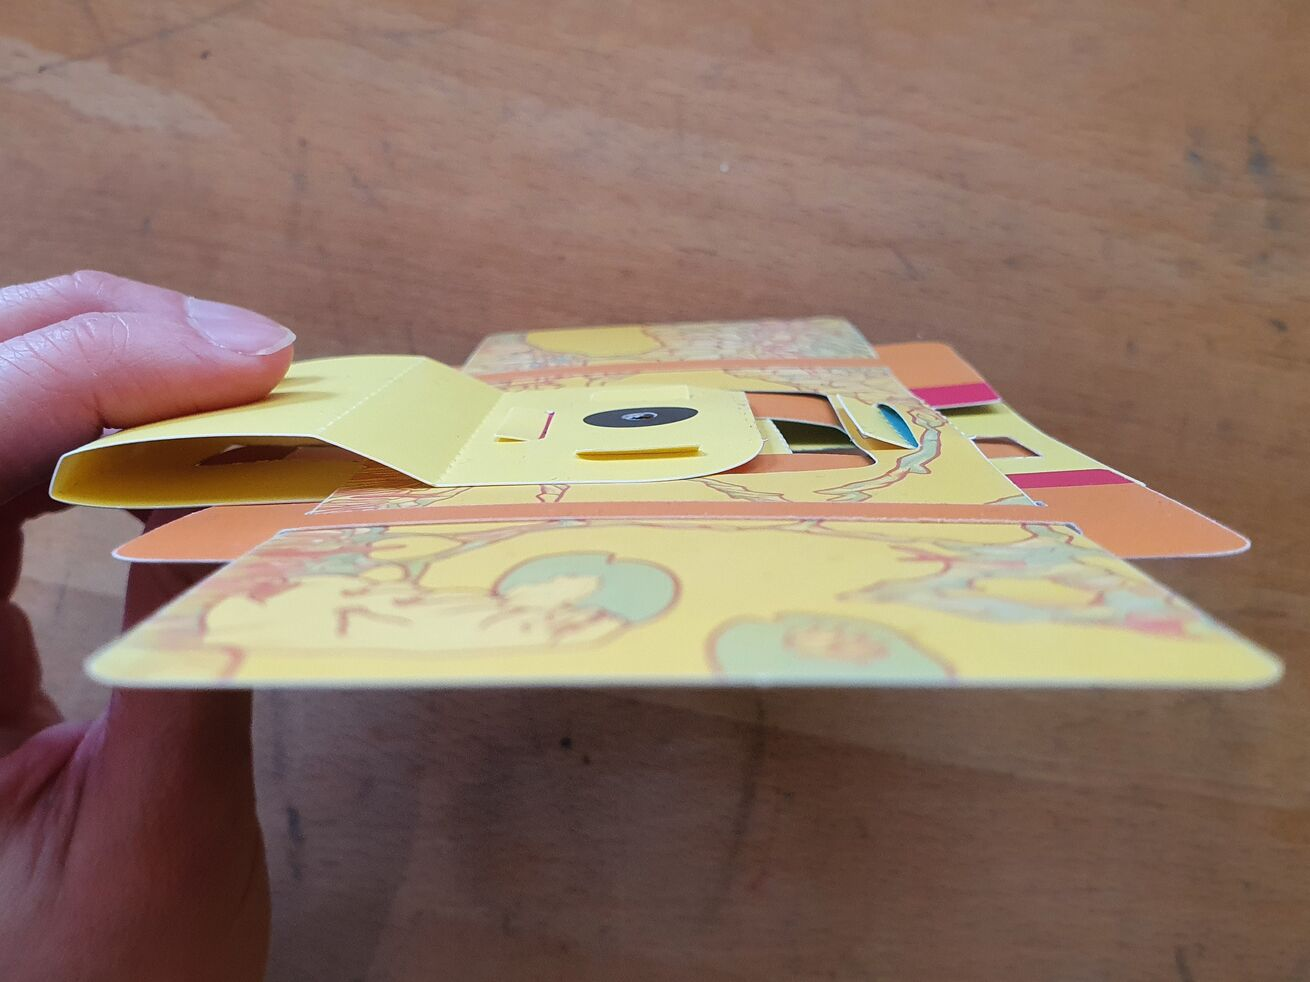
\includegraphics[width=0.3\textwidth]{images/aufbau/9.jpg} &
				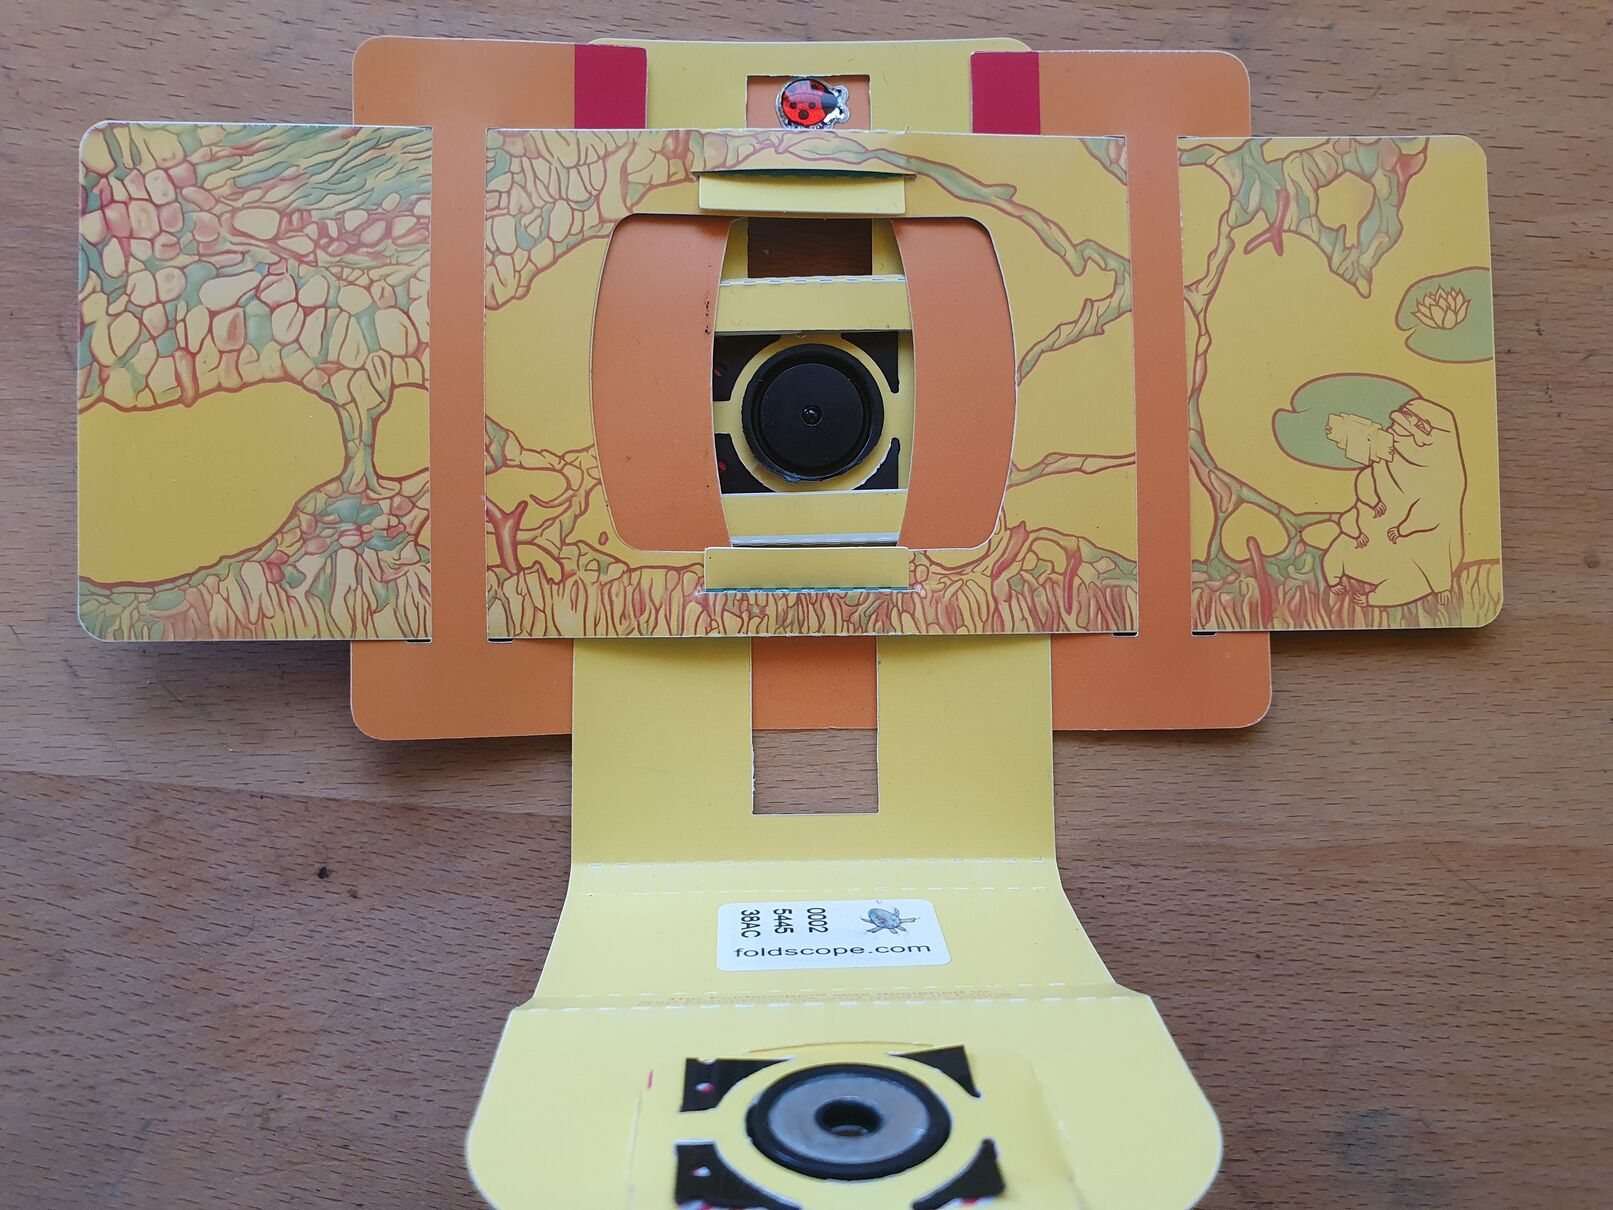
\includegraphics[width=0.3\textwidth]{images/aufbau/10.jpg} & 
				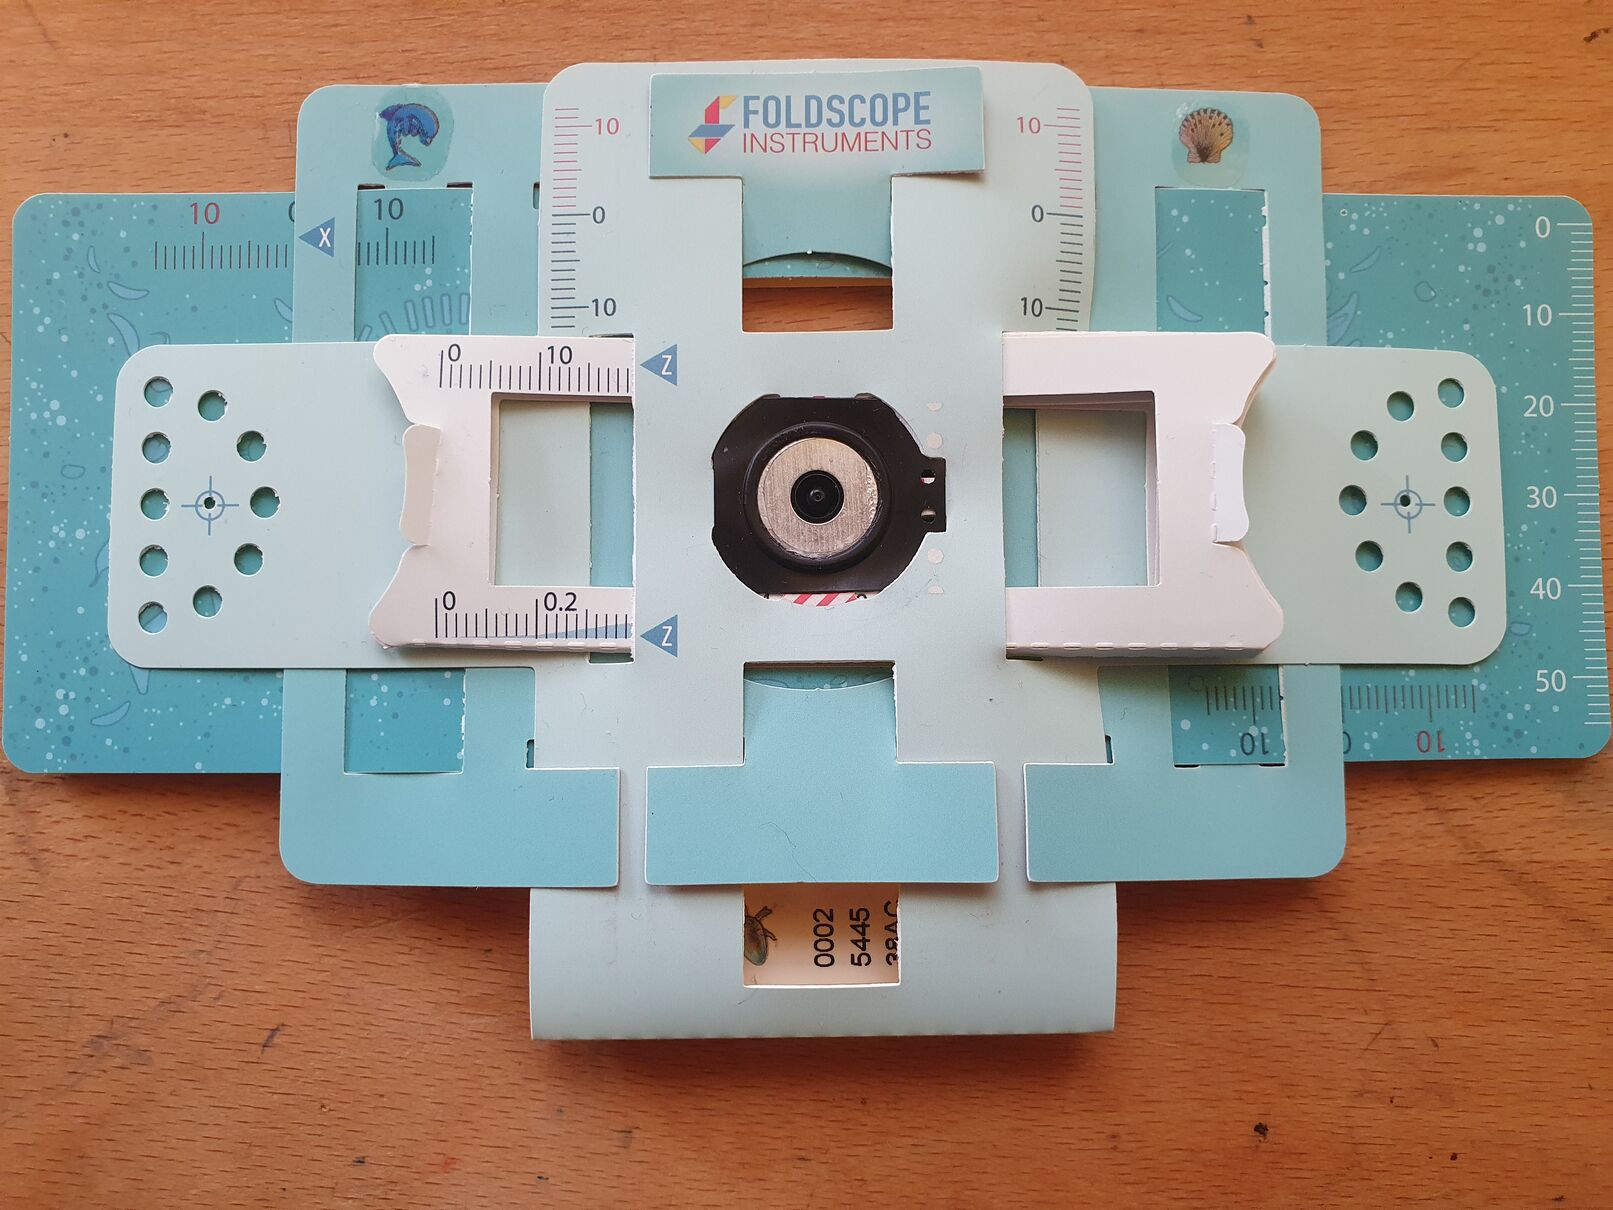
\includegraphics[width=0.3\textwidth]{images/aufbau/fertig.jpg} \\
				% \bottomrule
			\end{tabular}
		\end{center}
		\vspace{1em}
		Im Schritt 10 ("Foldscope individualisieren") haben wir zusätzlich mit Aufkleber unsere Foldscopes verziert. Mein fertiges Foldscope sieht dann so aus:
		\begin{figure}[H]
			\centering
			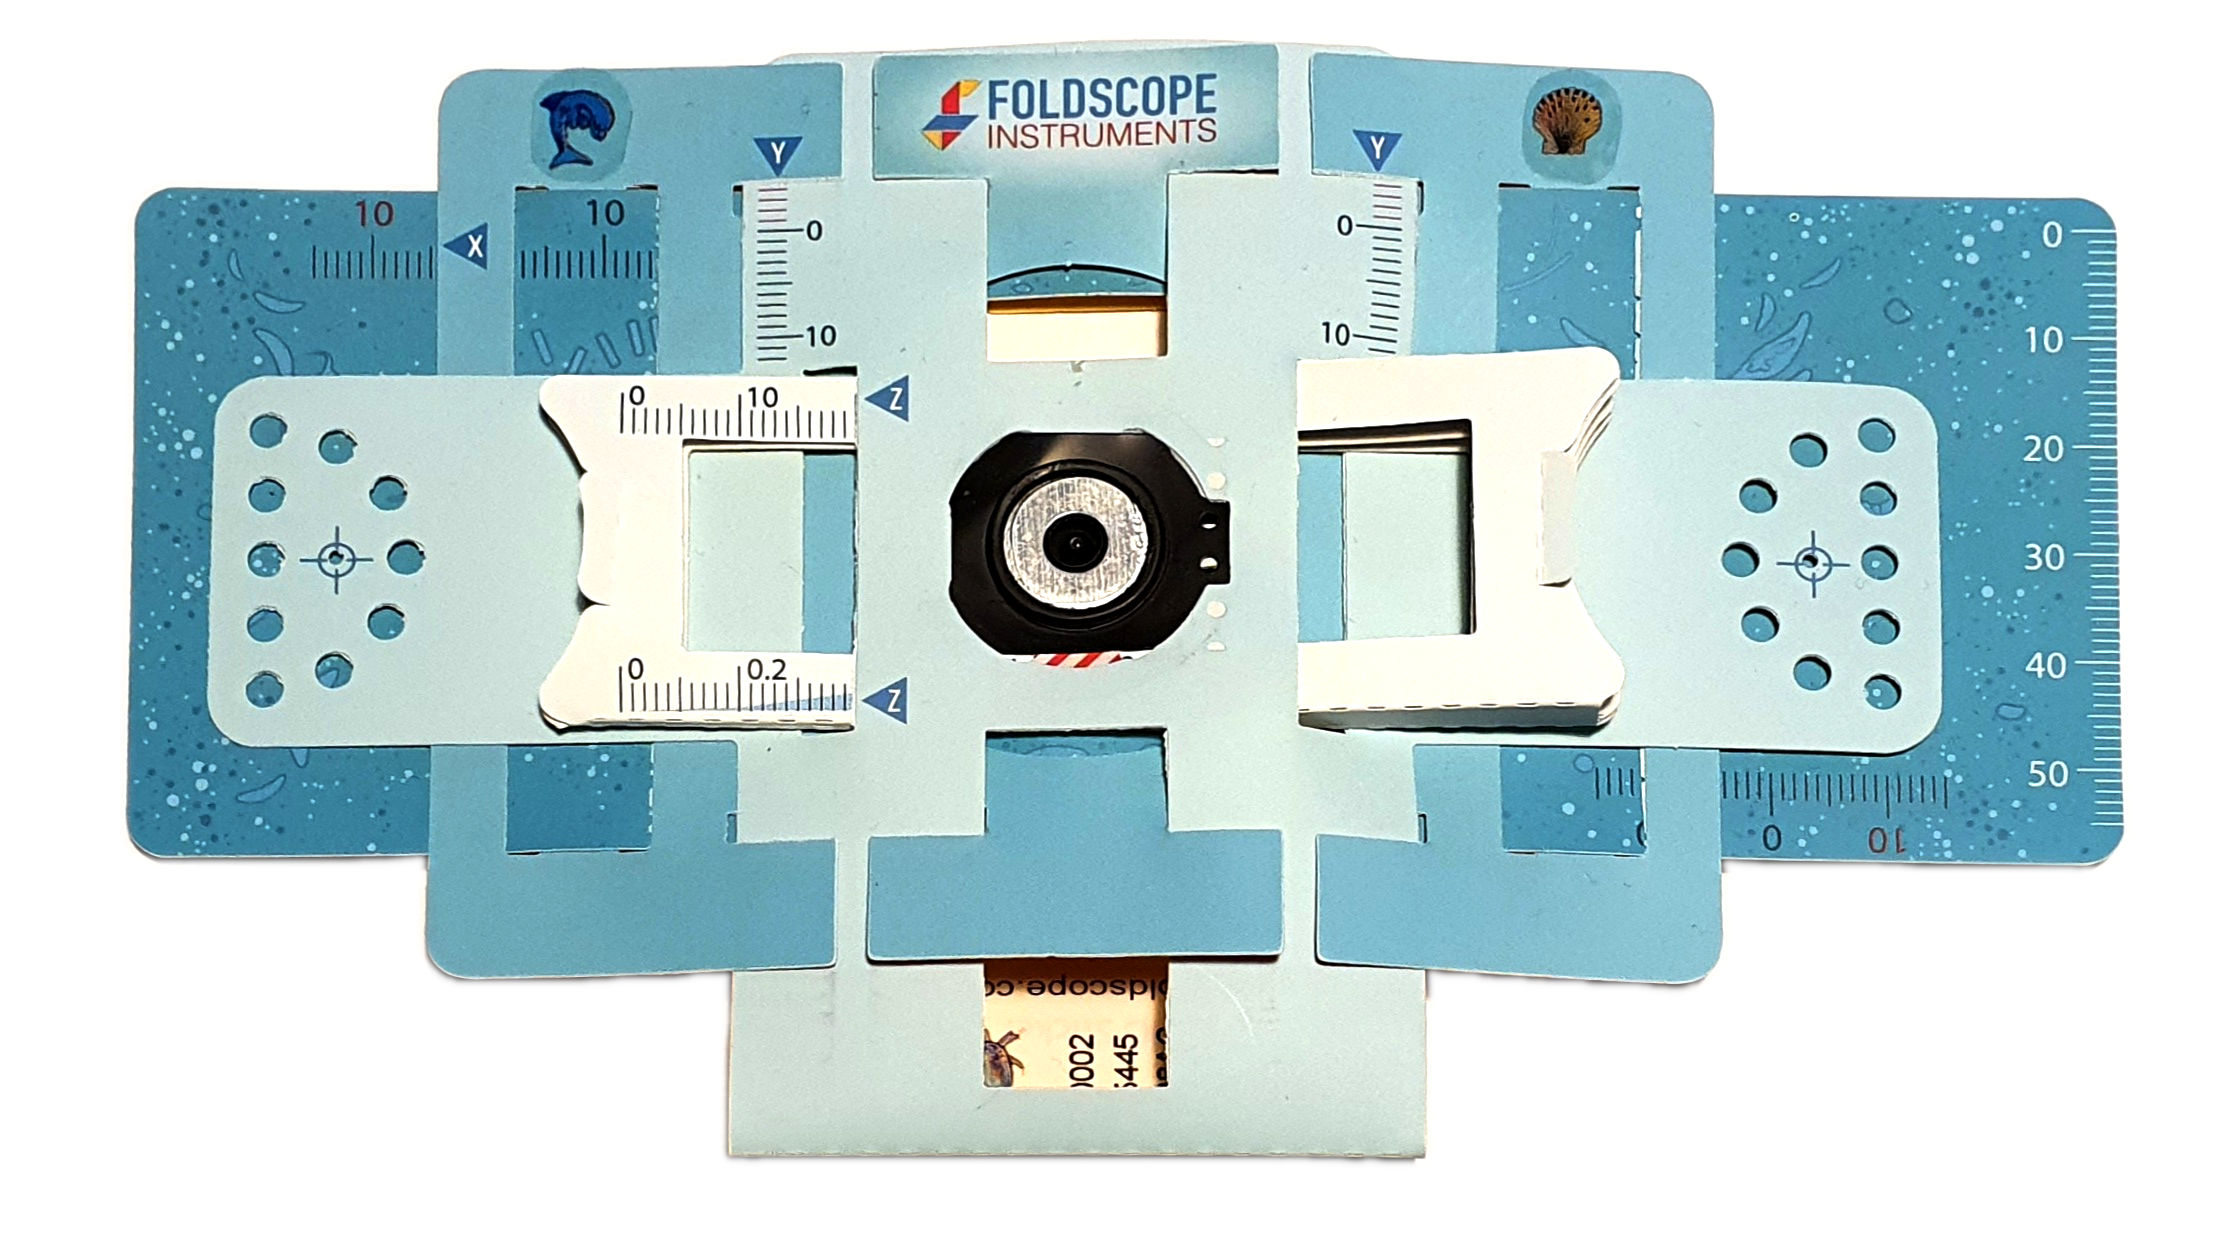
\includegraphics[width=0.6\textwidth]{cover.jpg}
			\caption{\centering Foldscope \texttt{0002} \texttt{5445} \texttt{38AC}}
		\end{figure}

\newpage 
\section{Teilversuch 2: Messung der Drehungswinkel der Polarisationsebene in Abhängigkeit vom Einfallswinkel}
	Wir setzen zunächst eine Vorzeichenkonvention fest: eine Drehung im Gegenuhrzeigesinn ist positiv und eine Drehung im Uhrzeigesinn ist negativ. Somit ist der Polarisator $P_1$ um $\delta = \SI{-45.0(5)}{\degree}$ eingestellt. Aus der Anleitung haben wir $\Psi = \delta - \omega$ mit 
	\begin{equation}
		\label{eqn:psi}
		\Psi = \arctan \left(- \frac{\cos\alpha \sqrt{n^2-\sin^2\alpha}}{\sin^2\alpha} \right)
	\end{equation}
	Wenn man die Gleichung \eqref{eqn:psi} für $n=\num{1.5}$ plottet, sieht man, dass bei $\alpha = \SI{0}{\degree}$, die Winkeländerung $\Psi \approx \SI{-90}{\degree}$ ist. Das ergibt auch Sinn, da die Händigkeit eines zirkular polarisierten Licht sich bei einer senkrechten Reflexion ändert. Wir wissen, dass diese Drehung im Gegenuhrzeigesinn sein soll, also stimmt dieses negatives Vorzeichen mit unserer Vorzeichenkonvention (da $\Psi = \delta - \omega \equiv \theta_\text{Initial} - \theta_\text{Final} = - (\theta_\text{Final} - \theta_\text{Initial})$). 

	Es ist hier auch zu bemerken, dass hier nur die Differenz zwischen $P_1$ und $P_2$ wichtig ist. In diesem Fall stimmen die Winkel hier nicht mit der Winkel aus der Anleitung. In der Anleitung ist der Winkel $\delta$ und $\omega$ von der $E^\parallel$-Achse gemessen. Im Experiment sind sie aber von der $E^\bot$-Achse gemessen. Also gilt mit der Anleitungkonvention:
	\begin{align}
		\delta &=  \SI{90}{\degree} - \SI{45.0(5)}{\degree} = \SI{45.0(5)}{\degree} \\ 
		\omega &=  (\SI{90}{\degree} - P_2)\,\brc{ + \SI{90}{\degree}~}{} = \SI{180}{\degree} - P_2 \\[-1em]
		&\phantom{=  \SI{90}{\degree}}\text{\scriptsize Gemessene $P_2$ senkrecht zur Polarisationsebene} \notag
	\end{align} 
	Im unserer Konvention ist aber mit einer Drehung im Gegenuhrzeigesinn:
	\begin{align}
		\delta &=  \SI{-45.0(5)}{\degree}\\ 
		\omega &=  -P_2 + \SI{90}{\degree}
	\end{align}
	In beiden Fälle ist die Vorzeichenkonvention gleich: Drehung im Gegenuhrzeigesinn $ = $ positiv.

	Daraus folgt, dass unseres $\Psi$ (und dessen Fehler) gegeben durch ist:
	\begin{align}
		\Psi &= \delta - \omega = \SI{-45.0}{\degree} - \left(-P_2 + \SI{90}{\degree}\right) = P_2 - \SI{135.0}{\degree} \\
		\Delta\Psi &= \addquad{\delta,\omega}
	\end{align}
	\begin{beispiel}
		Für $\alpha = \SI{15.0(25)}{\degree}$ ist:
		\begin{align}
			\Psi = \SI{46.0}{\degree} - \SI{135.0}{\degree} = \SI{-89.0}{\degree}
		\end{align}
	\end{beispiel}
	Die weitere Rechnungen erfolgen im LibreOffice Calc.
	\newpage
	Mit $\alpha = \frac{\varphi}{2}$:
	\begin{center}
		\begin{tabular}{l*{8}{r}}
			\toprule
			$\alpha / \si{\degree}$ & \num{15.0} & \num{20.0} & \num{25.0} & \num{30.0} & \num{35.0} & \num{40.0} & \num{45.0} & \num{50.0} \\
			\midrule
			$\Psi / \si{\degree}$   & \num{-89.0} & \num{-87.0} & \num{-84.5} & \num{-81.0} & \num{-76.5} & \num{-73.0} & \num{-67.0} & \num{-60.0} \\
			\bottomrule
			\\[-0.5em]
			\toprule
			$\alpha / \si{\degree}$ & \num{52.5} & \num{55.0} & \num{57.5} & \num{60.0} & \num{65.0} & \num{70.0} & \num{75.0} & \num{80.0} \\
			\midrule
			$\Psi / \si{\degree}$   & \num{-56.5} & \num{-52.0} & \num{-48.0} & \num{-43.0} & \num{-35.0} & \num{-25.0} & \num{-14.5} & \num{-11.0} \\
			\bottomrule
		\end{tabular}
	\end{center}
	mit $\Delta\Psi = \addquad{\delta,\omega} = \sqrt{2(\num{0.5}^2)} = \SI{0.8}{\degree}$. Es ist ein Fehler von $\Delta \alpha = \SI{2.5}{\degree}$ auch zu berücksichtigen.

	Nun plotten wir die Daten mit \gnuplot{} und führe eine Kurveanpassung mit Gleichung \eqref{eqn:psi} durch (siehe Appendix \ref{appdx:tv2-gnuplot}). Wie vorher ist $n = \num{1.55}$ als Anfangswert verwendet.
	\begin{figure}[H]
		\centering
		% GNUPLOT: LaTeX picture with Postscript
\begingroup
  \makeatletter
  \providecommand\color[2][]{%
    \GenericError{(gnuplot) \space\space\space\@spaces}{%
      Package color not loaded in conjunction with
      terminal option `colourtext'%
    }{See the gnuplot documentation for explanation.%
    }{Either use 'blacktext' in gnuplot or load the package
      color.sty in LaTeX.}%
    \renewcommand\color[2][]{}%
  }%
  \providecommand\includegraphics[2][]{%
    \GenericError{(gnuplot) \space\space\space\@spaces}{%
      Package graphicx or graphics not loaded%
    }{See the gnuplot documentation for explanation.%
    }{The gnuplot epslatex terminal needs graphicx.sty or graphics.sty.}%
    \renewcommand\includegraphics[2][]{}%
  }%
  \providecommand\rotatebox[2]{#2}%
  \@ifundefined{ifGPcolor}{%
    \newif\ifGPcolor
    \GPcolortrue
  }{}%
  \@ifundefined{ifGPblacktext}{%
    \newif\ifGPblacktext
    \GPblacktexttrue
  }{}%
  % define a \g@addto@macro without @ in the name:
  \let\gplgaddtomacro\g@addto@macro
  % define empty templates for all commands taking text:
  \gdef\gplbacktext{}%
  \gdef\gplfronttext{}%
  \makeatother
  \ifGPblacktext
    % no textcolor at all
    \def\colorrgb#1{}%
    \def\colorgray#1{}%
  \else
    % gray or color?
    \ifGPcolor
      \def\colorrgb#1{\color[rgb]{#1}}%
      \def\colorgray#1{\color[gray]{#1}}%
      \expandafter\def\csname LTw\endcsname{\color{white}}%
      \expandafter\def\csname LTb\endcsname{\color{black}}%
      \expandafter\def\csname LTa\endcsname{\color{black}}%
      \expandafter\def\csname LT0\endcsname{\color[rgb]{1,0,0}}%
      \expandafter\def\csname LT1\endcsname{\color[rgb]{0,1,0}}%
      \expandafter\def\csname LT2\endcsname{\color[rgb]{0,0,1}}%
      \expandafter\def\csname LT3\endcsname{\color[rgb]{1,0,1}}%
      \expandafter\def\csname LT4\endcsname{\color[rgb]{0,1,1}}%
      \expandafter\def\csname LT5\endcsname{\color[rgb]{1,1,0}}%
      \expandafter\def\csname LT6\endcsname{\color[rgb]{0,0,0}}%
      \expandafter\def\csname LT7\endcsname{\color[rgb]{1,0.3,0}}%
      \expandafter\def\csname LT8\endcsname{\color[rgb]{0.5,0.5,0.5}}%
    \else
      % gray
      \def\colorrgb#1{\color{black}}%
      \def\colorgray#1{\color[gray]{#1}}%
      \expandafter\def\csname LTw\endcsname{\color{white}}%
      \expandafter\def\csname LTb\endcsname{\color{black}}%
      \expandafter\def\csname LTa\endcsname{\color{black}}%
      \expandafter\def\csname LT0\endcsname{\color{black}}%
      \expandafter\def\csname LT1\endcsname{\color{black}}%
      \expandafter\def\csname LT2\endcsname{\color{black}}%
      \expandafter\def\csname LT3\endcsname{\color{black}}%
      \expandafter\def\csname LT4\endcsname{\color{black}}%
      \expandafter\def\csname LT5\endcsname{\color{black}}%
      \expandafter\def\csname LT6\endcsname{\color{black}}%
      \expandafter\def\csname LT7\endcsname{\color{black}}%
      \expandafter\def\csname LT8\endcsname{\color{black}}%
    \fi
  \fi
    \setlength{\unitlength}{0.0500bp}%
    \ifx\gptboxheight\undefined%
      \newlength{\gptboxheight}%
      \newlength{\gptboxwidth}%
      \newsavebox{\gptboxtext}%
    \fi%
    \setlength{\fboxrule}{0.5pt}%
    \setlength{\fboxsep}{1pt}%
\begin{picture}(8640.00,5760.00)%
    \gplgaddtomacro\gplbacktext{%
      \csname LTb\endcsname%%
      \put(682,704){\makebox(0,0)[r]{\strut{}$-5$}}%
      \put(682,1253){\makebox(0,0)[r]{\strut{}$0$}}%
      \put(682,1803){\makebox(0,0)[r]{\strut{}$5$}}%
      \put(682,2352){\makebox(0,0)[r]{\strut{}$10$}}%
      \put(682,2902){\makebox(0,0)[r]{\strut{}$15$}}%
      \put(682,3451){\makebox(0,0)[r]{\strut{}$20$}}%
      \put(682,4000){\makebox(0,0)[r]{\strut{}$25$}}%
      \put(682,4550){\makebox(0,0)[r]{\strut{}$30$}}%
      \put(682,5099){\makebox(0,0)[r]{\strut{}$35$}}%
      \put(814,484){\makebox(0,0){\strut{}$450$}}%
      \put(2052,484){\makebox(0,0){\strut{}$500$}}%
      \put(3290,484){\makebox(0,0){\strut{}$550$}}%
      \put(4529,484){\makebox(0,0){\strut{}$600$}}%
      \put(5767,484){\makebox(0,0){\strut{}$650$}}%
      \put(7005,484){\makebox(0,0){\strut{}$700$}}%
      \put(8243,484){\makebox(0,0){\strut{}$750$}}%
    }%
    \gplgaddtomacro\gplfronttext{%
      \csname LTb\endcsname%%
      \put(209,2901){\rotatebox{-270}{\makebox(0,0){\strut{}Anzahl der Durchgängen $\Delta m$ (Einheitslos)}}}%
      \put(4528,154){\makebox(0,0){\strut{}Druck $P$ ($\si{\hecto\pascal}$)}}%
      \csname LTb\endcsname%%
      \put(7256,1977){\makebox(0,0)[r]{\strut{}Messung 1}}%
      \csname LTb\endcsname%%
      \put(7256,1757){\makebox(0,0)[r]{\strut{}Messung 2}}%
      \csname LTb\endcsname%%
      \put(7256,1537){\makebox(0,0)[r]{\strut{}Messung 3}}%
      \csname LTb\endcsname%%
      \put(7256,1317){\makebox(0,0)[r]{\strut{}$0,12876P + (-63,61708)$}}%
      \csname LTb\endcsname%%
      \put(7256,1097){\makebox(0,0)[r]{\strut{}$0,12976P + (-65,87209)$}}%
      \csname LTb\endcsname%%
      \put(7256,877){\makebox(0,0)[r]{\strut{}$0,15166P + (-73,36752)$}}%
      \csname LTb\endcsname%%
      \put(4528,5429){\makebox(0,0){\strut{}Druck gegen die Anzahl der Durchgängen}}%
    }%
    \gplbacktext
    \put(0,0){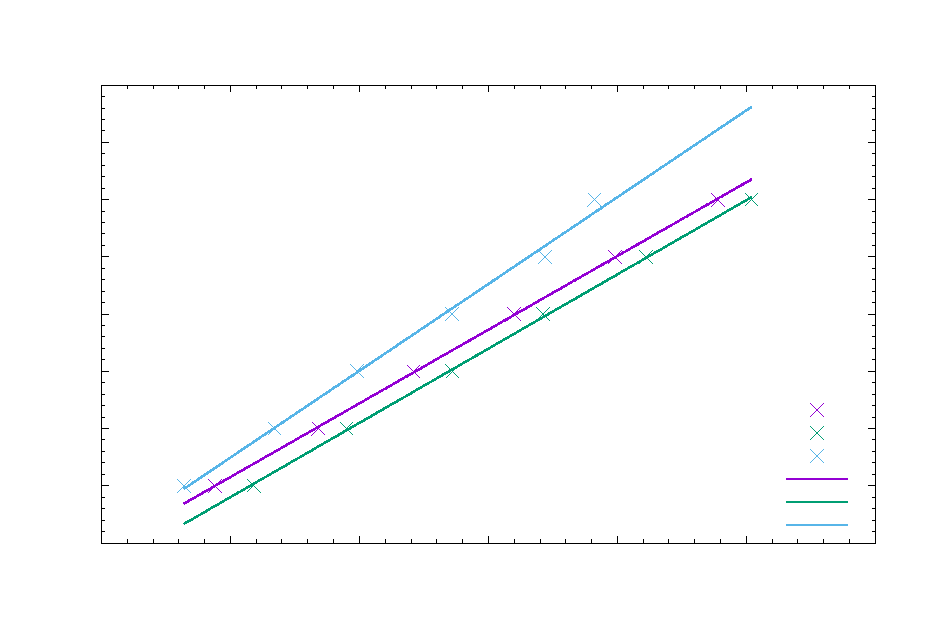
\includegraphics[width={432.00bp},height={288.00bp}]{tv2-plot}}%
    \gplfronttext
  \end{picture}%
\endgroup

		\caption{\centering Drehwinkel der Polarisationsebene gegen Einfallswinkel $(\chi^2_{\text{red}} = 0.609812)$ }
		\label{fig:tvtwo-plot}
		\vspace{-1em}
	\end{figure}
	Als Endergebnis erhalten wir: $n = \num{1.69105(4292)} = \num{1.69(5)}$. Die Anpassung hat ein $\chi^2_{\text{red}} = 0.609812 < 1$, was eine mögliche Überanpassung bedeuetet. Von unserem Plot ist aber klar, dass das nicht der Fall ist. Die Anpassung ist also eine gute Anpassung. 
	\newpage
	\subsection{Diskussion}
		Zusammengefasst haben wir:

		\begin{center}
			\vspace{0.5em}
			\begin{tabular}{ll}
				\toprule
				Methode & $n$ \\
				\midrule
				$\zeta^\bot$      & \num{1.465(7)} \\
				$\zeta^\parallel$ & \num{1.526(9)} \\
				$\alpha_p$        & \num{1.57(16)} \\
				\midrule
				Drehwinkel der Polarisationsebene & \num{1.69(5)} \\
				\midrule
				Anleitung         & \num{1.63} \\
				\bottomrule
			\end{tabular}
			\vspace{0.5em}
		\end{center}

		Der Brechungsindex, den wir im Teilversuch 2 berechnet haben, ist verträglich mit dem Literaturwert aus der Anleitung. Diese beide Werten unterscheiden sich nur knapp ($\num{0.01}$ außerhalb des Fehlerintervalls). Offentsichlich ist die Methode im Teilversuch 2 die genauere Methode, um die Brechungsindex zu berechnen. Da wir hier immer nur das Minimum gefunden haben, ohne es beachaten zu müssen, was die genaue Multimetermessung ist, ist dieser Methode von Raumbeleuchtung nur wenig betroffen. Es gab aber immer noch einen Unterscheid und die mögliche Fehlerquellen sind:
		\begin{itemize}
			\item Der Laserstrahl war nicht komplett horizontal (\textit{cf.} Teilversuch 1)
			\item Der Prismatisch muss bei jeder Messung erst vom Pfostenhalter freigesetzt werden, bevor man ihn drehen kann, was zur Ungenauigkeiten führen könnte. Die Endposition des Primas könnte deswegen nicht senkrecht zur Laserstrahl sein.
			\item Die Polarisationsfiltern standen eventuell nicht perfekt senkrecht zum Laserstrahl, was die Strahlrichtung und Polarisation eventuell ändern könnte.
			\item Bei mancher Winkel war es den genaue Winkel $\alpha$ wegen Parallexfehler unter einer unter einer Schraube schwer zu treffen. 
		\end{itemize}
		Um die Genauigkeit zu verbessern könnte man beispielsweise eine Postklammer verwendet werden, sodass man die Tischebene erhalten bleibt während man den Prismatisch dreht. 



\newpage
\newcommand*{\ncot}[0]{n_{\text{CO}_2}}

\section{Teilversuch 3: Bestimmung des Brechungsindex von $\text{CO}_2$}
	Aus der Anleitung ist der Brechungsindex von $\text{CO}_2$ gegeben durch:
	\begin{equation}
		\ncot = \nluft + \frac{N\lambda}{2l} \equiv \nluft + \varepsilon
	\end{equation}
	mit dem entsprechenden Fehler:
	\begin{align}
		\Delta \ncot &= \addquad{\nluft, \varepsilon} \notag \\
		&=\sqrt{(\Delta\nluft)^2 + \varepsilon^2 \left[
			\left(\frac{\Delta N}{N}\right)^2 + 
			\left(\frac{\Delta \lambda}{\lambda}\right)^2 + 
			\left(\frac{\Delta l}{l}\right)^2
		\right]}
	\end{align}
	Aus dem Versuch haben wir einen Durchschnitt von $N = \num{12(1)}$, wobei $\Delta N = 1$ die Schwankung ist. Die Schwankung ist hier als Unsicherheit genommen, da $n=3$ zu klein einer Datensatz ist, um die statische Unsicherheit als Unsicherheit zu betrachten.

	Mit der Werten:
	\begin{center}
		\begin{tabular}{lll}
			\toprule
			Variable & Wert & Bedeutung \\
			\midrule
			$\lambda$ & \SI{520(20)}{\nano\meter} & Wellenlänge des Lasers \\
			$l$ & \SI{50(1)}{\milli\meter} & Optische Länge der Kapsel \\
			$\nluft$ & \num{1.00(10)} & Brechungsindex von Luft \\
			$N$ & \num{12(1)} & Durchschnittliche Anzahl von Durchgänge \\
			\bottomrule
		\end{tabular}
	\end{center}
	erhalten wir:
	\begin{align}
		\ncot  &= \num{1.00} + \frac{12(\SI{520e-9}{\meter})}{2(\SI{50e-3}{\meter})} = \num{1.0000624} \\
		\Delta\ncot
			&= \sqrt{(\num{0.10})^2 + \left(\num{6.24e-5}\right)^2 \left[
				\left(\frac{1}{12}\right)^2 + 
				\left(\frac{20}{520}\right)^2 + 
				\left(\frac{1}{50}\right)^2
			\right]} \notag \\
			&= \num{0.11} \sigfig{2}
	\end{align}
	Somit ist $\ncot = \num{1.00(11)}$, was mit dem Litaturwert von $n_{\text{CO}_2\text{, Lit}} = \num{1.000416}$ übereinstimmt. Unserer Mach-Zender-Interferometer ist aber einfach zu ungenau, um ein besseres Ergebnis zu erhalten. 

\resnum
\newpage
\appendix
\section{Anleitung zur Foldscope}
    \label{appdx:anleitung}
    \begin{center}
        \vfill
        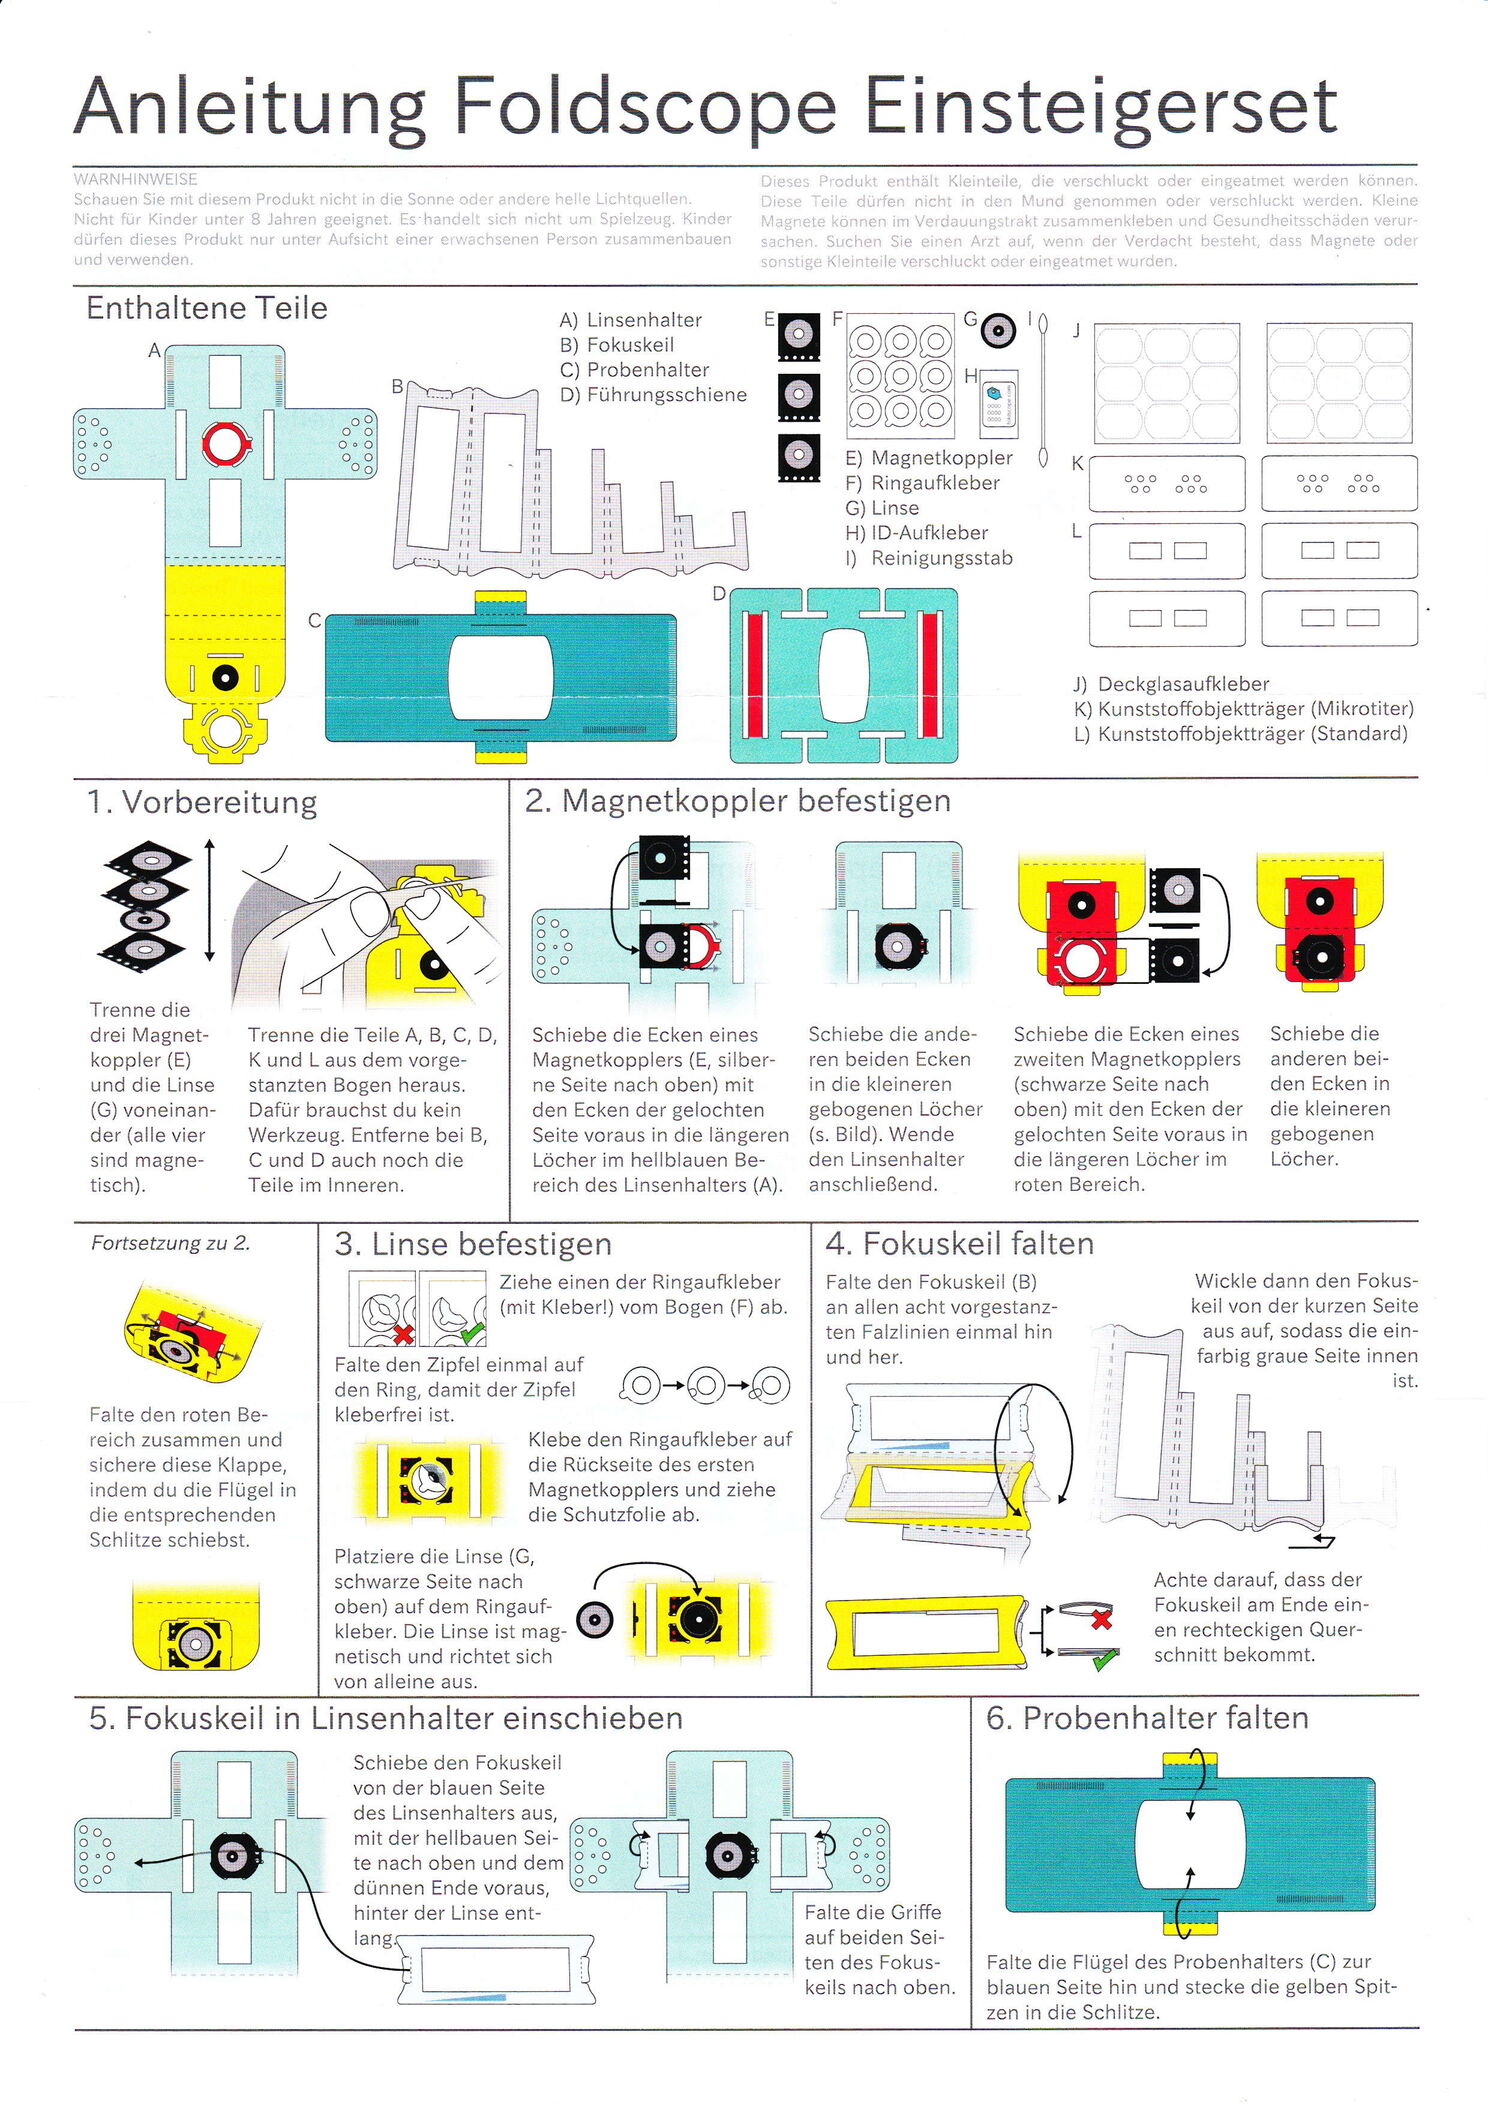
\includegraphics[width=0.91\textwidth]{page-000.jpg}
        \vfill
    \end{center}
    \begin{center}
        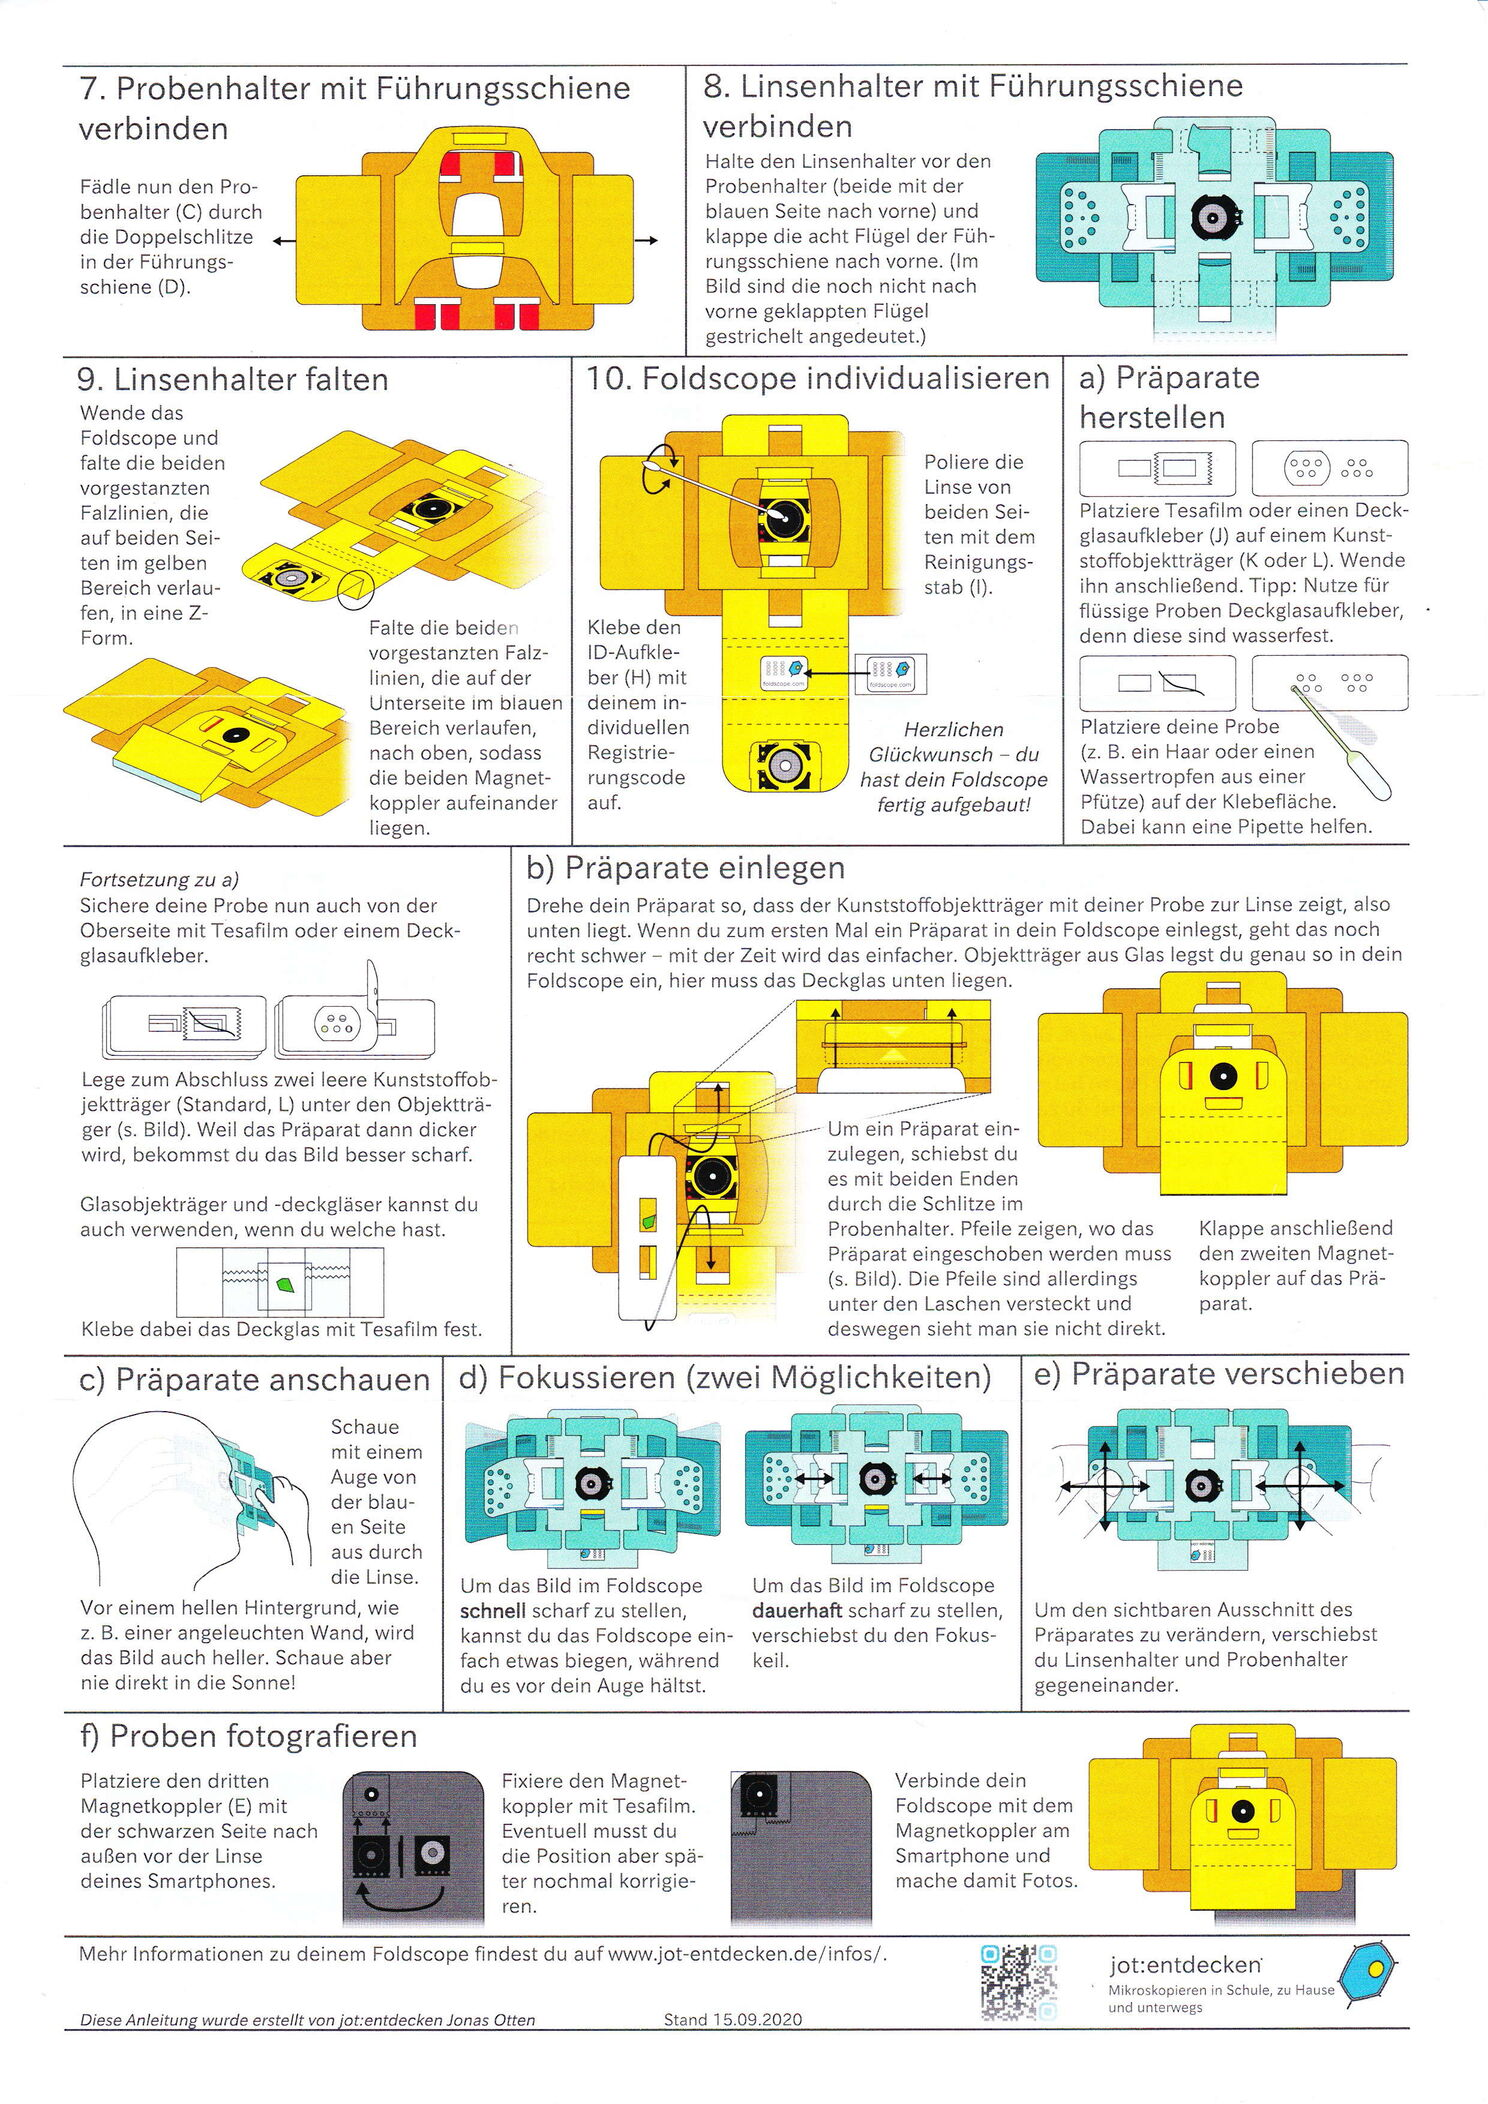
\includegraphics[width=\textwidth]{page-001.jpg}
    \end{center}
\end{document}
